%%
%% This is file `./samples/longsample.tex',
%% generated with the docstrip utility.
%%
%% The original source files were:
%%
%% apa6.dtx  (with options: `longsample')
%% ----------------------------------------------------------------------
%% 
%% apa6 - A LaTeX class for formatting documents in compliance with the
%% American Psychological Association's Publication Manual, 6th edition
%% 
%% Copyright (C) 2011-2014 by Brian D. Beitzel <brian at beitzel.com>
%% 
%% This work may be distributed and/or modified under the
%% conditions of the LaTeX Project Public License (LPPL), either
%% version 1.3c of this license or (at your option) any later
%% version.  The latest version of this license is in the file:
%% 
%% http://www.latex-project.org/lppl.txt
%% 
%% Users may freely modify these files without permission, as long as the
%% copyright line and this statement are maintained intact.
%% 
%% This work is not endorsed by, affiliated with, or probably even known
%% by, the American Psychological Association.
%% 
%% ----------------------------------------------------------------------
%% 
\documentclass[man]{apa6}


\usepackage{apacite}
\usepackage{todonotes}
\usepackage{booktabs}
\usepackage{url}
%\usepackage{gb4e}

\usepackage{amsmath,epsfig}

%\usepackage[american]{babel}

\usepackage{csquotes}
%\usepackage[style=apa,sortcites=true,sorting=nyt,backend=biber]{biblatex}
%\DeclareLanguageMapping{american}{american-apa}
%\addbibresource{bibliography.bib}

\title{Formalizing the Pragmatics of Figurative Language}
\shorttitle{Formalizing the Pragmatics of Figurative Language}

\threeauthors{Justine T. Kao}{Leon Bergen}{Noah D. Goodman}
\threeaffiliations{Stanford University}{Massachusetts Institute of Technology}{Stanford University}


\leftheader{Kao}

\abstract{People often use language to convey information that goes far beyond an utterance's literal meaning. In particular, figurative language such as hyperbole, irony, and metaphor showcase people's ability to use background knowledge and social reasoning to interpret utterances in context.
% and context to derive linguistic meaning.
%For example, metaphors highlight specific similarities between disparate concepts; hyperbolic statements communicate speakers� attitudes and opinions without explicitly stating them. 
While figurative utterances are often literally false, people are highly adept at inferring relevant and true information from these utterances. What is the cognitive and linguistic basis of figurative language understanding?
%People routinely go beyond the literal meanings of utterances to infer speakers' intended meanings in context. In particular, figurative language such as hyperbole, irony, and metaphor showcase people's ability to use background knowledge and context to derive linguistic meaning.
%Although figurative language is prevalent in human communication, how people arrive at appropriate interpretations of figurative utterances remains unclear.
%using contextual and background information
Here we describe a computational model that formalizes figurative communication as recursive social reasoning between speaker and listener. Our model extends and overcomes limitations of basic Rational Speech Act (RSA) models, a family of computational models that capture many phenomena in human pragmatic reasoning but are restricted to the interpretation of literally true utterances.
%Our model incorporates uncertainty about the speaker's communicative goal, otherwise known as the question under discussion (QUD). 
We show that an RSA model extended to accommodate inferences about the topic of conversation is able to predict people's interpretations of hyperbole, irony, and metaphor. We argue that despite apparent differences among these subtypes of figurative language, the same computational framework flexibly produces fine-grained interpretations for a range of figurative uses. We use this as evidence suggesting that the rich and often affectively-laden meanings expressed by figurative language can be explained by basic principles of communication.
%Understanding others' thoughts through the words they speak requires integrating a host of information sources to create meaning. figurative language  --- sentences whose intended meanings differ significantly from their literal meanings --- raises questions about the linguistic, cognitive, and social faculties that enable people to go beyond linguistic input and reason about others' intentions in understand utterances in context. 

%My research uses figurative language as a case study to examine how listeners integrate common knowledge and social reasoning to infer speakers' communicative intents when interpreting utterances.
%I combine behavioral experiments and computational modeling to 
%investigate the shared principles underlying diverse types of figurative language such as hyperbole and metaphor. In addition, I apply tools from information theory and natural language processing to investigate downstream effects of creative language such as humor and poetic beauty.
%\textbf{By incorporating experimental and computational methods to examine creative language use, my research 
%advances our knowledge of how people derive socially meaningful information from language
%%unifies diverse types of figurative language under the same formal pragmatic framework 
%and introduces rigor to theories of communication.}
}

\keywords{pragmatics, figurative language, computational modeling}

\authornote{Justine T. Kao, Department of Psychology,
  Stanford University.
  
  Leon Bergen, Department of Brain and Cognitive Sciences, MIT.
  
  Noah D. Goodman, Department of Psychology, Stanford University.

  Correspondence concerning this article should be addressed to Justine T. Kao, Department of Psychology, Stanford University, 450 Serra Mall, Stanford, CA 94025.  E-mail: justinek@stanford.edu}

\begin{document}
\maketitle
The ability to understand figurative language is necessary in a world where people do not always mean what they say. We implicate, exaggerate, make metaphors, and wax poetic. 
From ``Juliet is the sun'' to ``It took a million years to write this paper,'' figurative language such as metaphor, irony, and hyperbole are commonplace in everyday communication, creating poetic or humorous effects that add richness and interest to linguistic behavior \cite{glucksberg2001understanding, pilkington2000poetic, lakoff2009more, roberts1994people}. 
%People often use language to convey information that goes far beyond a sentence's literal meaning. Hyperbolic statements communicate speakers' attitudes and opinions by exaggerating the truth (``It took a million years to write this paper''); ironic or sarcastic statements communicate meanings contrary to what is encoded in the literal semantics (``Paper-writing is my favorite activity''); and metaphors highlight hidden similarities between distinct categories by equating them (``Paper-writing is a marathon''). 
Although figurative statements are often false under their literal semantics (Juliet is not literally the sun, and it is infeasible to take a million years to write a paper), people are highly adept at inferring relevant and true information from these utterances (e.g. Romeo thinks Juliet is beautiful; it took unexpectedly long to write this paper). Because the literal meanings of these utterances are insufficient for uncovering the intended meanings, understanding figurative language requires integrating a host of information sources to create meaning, a hallmark of human intelligence that underlies many aspects of how we understand and interact with the world. How do our linguistic, cognitive, and social faculties work together to allow us to fluently and accurately understand the communicative intent behind figurative utterances?

An ocean of ink has been spilled across many disciplines to answer this question, including psychology, linguistics, philosophy, computer science, and literary theory \cite{glucksberg2001understanding, papafragou1996figurative, li2010using, kreuz1993empirical}.  Much of the  empirical research on figurative language focuses on cognitive mechanisms that underly interpretations of specific types of figurative use. For example, researchers have proposed various ways in which people align shared properties and analogous relations across different domains in order to understand metaphor, including the domain interaction model \cite{tourangeau1982understanding}, structure mapping model \cite{gentner1997alignment, gentner1983structure}, and category assertion model \cite{glucksberg2003psycholinguistics}. To explain a different type of figurative language such as verbal irony, researchers then posit separate mechanisms such as pretense \cite{clark1984pretense} or echoic mention \cite{sperber1981irony} to address the specific factors that shape ironic interpretations. While these approaches significantly advance our understanding of the conceptual factors that guide metaphor and irony understanding, they tend to treat each type of figurative language as requiring a separate mechanism distinct from or in addition to standard language understanding. By relying on a more specialized mechanism for figurative language, these approaches leaves open the question of how utterances such as ``My surgeon is a butcher'' or ``Such lovely weather we're having'' (uttered in the middle of a storm) trigger these particular mechanisms in the first place.
%, or why, if figurative utterances require an additional processing step, it is often just as easy to understand these utterances as their literal paraphrases in certain contexts.

A different approach to studying figurative language focuses on how people use general communicative principles to arrive at contextually appropriate interpretations \cite{grice20134, searle1979metaphor, sperber2008deflationary, ortony1993metaphor, tendahl2008complementary}. Two main views in the pragmatics literature have taken this view to examine figurative language: the standard pragmatic view and the relevance theoretic view. The standard pragmatic view analyzes figurative utterances using the cooperative principle and standard Gricean maxims, which state that speakers tend to produce utterances that adhere to principles of quality (truthfulness), quantity (informativeness), relevance, and manner (e.g. brevity, orderliness, clarity) \cite{grice20134, searle1979metaphor}. Under this view, figurative utterances are understood through a three-step process: (1) determine the literal meaning of the utterance (2) determine whether the literal meaning violates the quality maxim by being untruthful (3) reanalyze the utterance to identify implied or figurative meanings that would allow the utterance to adhere to the Gricean maxims. Although the standard pragmatic view is appealing in that it fits naturally within a more general theory of pragmatics, it has met with several criticisms. One of them is the fact that many figurative statements do not violate the quality maxim because their literal meanings can also be true. ``No man is an island,'' for example, is a literally true statement (there does not exist a man that is literally a piece of land surrounded by water) in addition to a metaphorically meaningful one (people do not exist in isolation) \cite{gibbs1992metaphor}. By relying on the violation of the quality maxim, the standard pragmatic view does not provide a satisfying explanation for how figurative meanings arise from these types of utterances. Another common criticism in the psycholinguistics literature is that the standard pragmatic view requires the listener to first access the literal meaning of the utterance, verify that the literal meaning is false, compute potential figurative interpretations, and then select the interpretation that best satisfies conversational maxims. Given the extra steps involved, this model would predict that people should take longer to interpret figurative utterances than literal utterances. However, many experiments have shown that the figurative meanings of irony and metaphor can be accessed as quickly or even more quickly than their literal meanings given supporting contexts \cite{glucksberg2003psycholinguistics, gildea1983understanding, gibbs1992metaphor}. These empirical findings suggest that literal meanings do not have to be explicitly computed and then rejected before appropriate figurative interpretations emerge.

A second view on the pragmatics of figurative language stems from relevance theory, a general theory of communication whose central claim is that human cognition is governed by a tendency to maximize relevance
\cite{sperber1986relevance}. 
\citeA{sperber2008deflationary} introduced the communicative principle of relevance, which is that ``every act of inferential communication conveys a presumption of its own optimal relevance.''
Instead of using Grice's four maxims as the guiding principle for figurative interpretation, relevance theory proposes that the principle of relevance is sufficient for explaining a range of phenomena in communication and cognition more generally. 
More specifically, the interpretation of all language involves maximizing the relevance of the interpretation to a contextually determined topic \cite{sperber2008deflationary, tendahl2008complementary}. As a result, interpretations of the same utterance can vary dramatically given different topics. Suppose two interlocutors, Ann and Bob, are discussing their friend Cam. Ann asks, ``Does Cam have a fever?'' and Bob replies, ``He is boiling.'' Ann will interpret Bob's utterance to mean that Cam has a very high temperature. If, on the other hand, Ann asks, ``Is Cam upset?'' and Bob replies, ``He's boiling,'' Ann should interpret Bob's utterance to mean that Cam is very angry. The word ``boiling'' receives different figurative meanings in these two contexts: in the first, Cam is very hot but not literally at boiling point; in the second, Cam is experiencing intense anger. Ann arrives at the appropriate interpretation by assuming that Bob's utterance provides maximally relevant information regarding her question. Under the relevance theoretic view, figurative uses such as hyperbole and metaphor are not distinct from literal language, but rather lie on a continuum of ``loose uses'' that all require listeners to use the principle of relevance to recover the intended meanings. This view situates figurative language within a general  theory of communication and has been argued to provide a complementary perspective to cognitive linguistics in the study of metaphor \cite{tendahl2008complementary}. However, one concern with relevance theory is that the concept of relevance, while intuitively appealing, has not been clearly operationalized or tested in a quantitative manner to determine its specific role in figurative language understanding. 

Taking the approach of analyzing general communicative principles that shape interpretations of figurative language, our goal in this paper is to propose an explicit and testable theory of figurative language understanding that can be validated against empirical data. We describe a computational model that integrates several pragmatic elements (e.g. assumptions that speakers are rational and cooperative; assumptions that utterances tend to be informative and relevant to the topic of conversation; representations of common knowledge and prior beliefs; and inferences about speakers' subjective attitudes) to produce appropriate interpretations of figurative utterances. In what follows, we first review core empirical phenomena in figurative language and highlight existing research and open questions regarding factors that shape figurative language understanding. Next, we will describe the ways in which many of these factors can be integrated through a framework of pragmatic reasoning. We introduce Rational Speech Act (RSA) models, a family of computational models that formalize communication as recursive social reasoning. We then show that natural but critical extensions can be made to RSA models to account for figurative language. We adapt the extended model to three types of figurative language: hyperbole, verbal irony, and metaphor, and present behavioral data and modeling results. Finally, we discuss the insights this model reveals about figurative language understanding as well as future research that our modeling approach licenses. We argue that a general model of figurative language enables us to more precisely examine the ways in which semantics and principles of communication interact to generate rich linguistic meaning.

%\section{A proposal}

%In the next chapter, I will describe such a formal model and argue that it may illuminate our understanding figurative communication.
%
%
%ARGUE FOR NOT ENOUGH EXPLICITNESS.
%While both the standard pragmatic and relevance theoretic view provide useful frameworks for understanding the pragmatics of figurative communication, certain factors that are important in general communication remain underspecified. For example, while relevance theory considers which interpretations are maximally relevant to the question under discussion, it does not provide a clear operationalization of relevance. 
%
%neither the standard pragmatic nor relevance theoretic view explicitly take into account the speaker's desire to be informative. There is also little consideration of the shared encyclopedic knowledge associated with different utterances, or representation of the listener's prior beliefs. WWe believe that an adequate model of figurative language understanding should flexibly integrate these components to determine an appropriate interpretation. In addition, figurative language is often used to  express subjective experiences and emotional attitudes \cite{riloff2005exploiting, roberts1994people}.
%Since these emotional subtexts contribute greatly to the appeal of figurative language, it is important for a theory of figurative language understanding to include analyses of these effects.
%
%Here we adopt an approach closer to the latter, with the goal of proposing a general pragmatic framework that explains the basis of figurative communication.


\section*{Figurative Language: The Phenomena} 
%\todo{include list of types of figurative language?}
Figurative language is often defined as utterances whose intended meanings differ in various ways from their ``literal'' or standard meanings \cite{gibbs1999figurative, gibbs2012interpreting}. 
%Under this definition, an utterance such as ``That chocolate cake is to die for'' is figurative, because the speaker does not mean that the chocolate cake is literally worth giving up one's life. Perhaps less obviously, an indirect speech act such as ``Can you pass the salt?'' is also figurative, because the intended meaning of the utterance differs from the literal meaning of the question---the speaker does not mean to inquire about the listener's ability to pass the salt.
At first glance, this definition seems straightforward and corresponds with our intuitions regarding which usages of language are literal and which are figurative. However, it quickly grows murky upon closer inspection. Suppose a speaker Bob says, ``I arrived late and the theater was full.'' Since it is implausible that the entire space of the theater was occupied from floor to ceiling, the sentence's strict literal meaning appears to be false. Instead, Bob most likely intends to communicate that he had difficulty finding an empty seat at the theater. This is an example of ``loose talk,'' also described as pragmatic slack, where a speaker uses a proposition $Q$ (e.g. the theater was full) in order to communicate a set of propositions that can be derived from $Q$ (e.g. there were a lot of people at the theater, and Bob was unable to find a seat), without being committed to the truthfulness of $Q$ \cite{sperber1985loose, lasersohn1999pragmatic, bach1994semantic}. 
%Based on the naive definition of figurative language, the utterance ``The theater was full'' can be characterized as not strictly literal and thus figurative.
%A speaker wishes to communicate a set of propositions $P_1 \dots P_n$ (e.g. there were a lot of people at the auditorium; we weren't able to find seats), which are derivable from a stricter proposition $Q$ (e.g. the auditorium was full). In order to minimize effort while effectively communicating $P_1 \dots P_n$, the speaker chooses to utter $Q$ without fully committing to its truth. Relevance theorists argue that the relevance principle---the assumption that speakers choose utterances to maximize relevance---is what allows listeners to correctly infer $P_1 \dots P_n$ without necessarily believing that $Q$ \cite{sperber1985loose}.
 
On the other hand, consider an utterance such as, ``Bob is always late,'' produced by an annoyed speaker. In order for the literal meaning of the utterance to be true, for all cases in which Bob can be either late or on time, Bob must be late in $100\%$ of the cases. However, one can easily interpret the utterance to mean that the speaker thinks Bob is very often (but not literally always) late, thus arriving at an interpretation that differs from the literal meaning of the utterance.
Under these analyses, the intended meanings of both utterances (``The theater was full'' and ``Bob is always late'') differ from their ``literal'' meanings. Indeed, \citeA{sperber1985loose} claim that there is no discontinuity between loose and figurative uses of language; both exploit the principle of relevance in order to express what is derivable from the utterance without committing to the truth of the literal meaning of the utterance. At the same time, a sentence such as ``Bob is always late'' feels qualitatively different from a sentence such as ``The theater was full'' and is more easily recognized as hyperbole. In fact, it has been observed that some utterances are intuitively recognized as ``figurative'' while other are not \cite{coulson2005blending}, which suggests that figurative language may be a psychologically meaningful category distinct from most other loose uses.

One characterization of this distinction is that figurative utterances are often used with the intention of producing particular effects and in order to accomplish discourse goals beyond relaying objective information about the world.   \citeA{roberts1994people} examined the discourse goals that motivate people to use various figurative tropes and identified a taxonomy of $19$ discourse goals, such as to convey emotion, to emphasize, to be humorous, or to be eloquent. 
\citeA{colston1998you} showed that hyperbole and irony are often used to express surprise. In addition, hyperbole and irony are more often used with friends and may signal social intimacy between speaker and listener \cite{blahblah} \todo{add bib}. Other work has shown that verbal irony can heighten or soften criticism \cite{colston1997salting}, elicit emotional reactions \cite{leggitt2000emotional}, highlight group membership \cite{gibbs2000irony}, and express affective attitudes \cite{colston1998you}.
Still other researchers have suggested that metaphors are often used to express subjective attitudes towards the subject \cite{ortony1979beyond}, and that subjective sentences frequently contain figures of speech such as metaphor and hyperbole \cite{riloff2005exploiting}. 
\todo{elaborate}
It is possible that the intuitive judgment of figurativeness involves recognizing that the speaker's intent is not to communicate objective information about the world, but rather to produce one or more of these rhetorical effects. 
As a result, it may be important to consider the affective subtexts and social information that figurative language communicates above and beyond most loose uses of language. 

%The definition of figurative language is further complicated when taking polysemy into account \cite{gibbs2012interpreting}. Consider the different senses of the word ``full.'' Suppose someone says, ``I am full'' after a meal. Since the speaker does not mean that the space inside her body is literally filled up, the sentence is not true under one particular literal meaning of ``full.'' However, one might argue that ``full'' has several different senses, and that the sense of being satisfied with food is the sense that is used literally in this utterance. One could then further modify the literal semantics of ``full'' for an utterance such as ``My heart is full (of emotion),'' such that the literal meaning of ``full'' includes a physical sensation in one's chest that roughly corresponds to experiencing emotion. In other words, one could keep adding different senses to the literal meaning of words until no usage is ever figurative. 
%Once one becomes sufficiently careful, it appears that the boundary between literal and figurative language is extremely fuzzy. At the same time, the fact that a great deal of research has targeted figurative language as a distinct category of language use, and that some utterances are intuitively recognized as ``figurative'' while other are not \cite{coulson2005blending}, suggests that such figurative language is a psychologically meaningful category. 
%%Where does this intuitive sense of ``figurative-ness'' come from? Do sentences have well-defined literal meanings, and is the distinction between literal and figurative meanings psychologically meaningful?  
%Instead of seeking to define the precise boundary between literal and figurative meanings, here we propose a weaker and less controversial definition. We suggest that the ``figurativeness'' of an utterance depends upon how Perhaps this intuition is based not on a clearcut boundary between literal and figurative meanings, but rather on a graded \emph{distance} between interpretations that the same utterance generates. Consider an utterance such as ``His car cost ten thousand dollars.'' Given most contexts that one can easily bring to mind, a reasonable interpretation of this utterance is that the car cost exactly $\$10,000$, or the car cost approximately $\$10,000$, and it is difficult to come up with a third interpretation. These two interpretations are not very different from each other. However, consider an utterance such as ``His cup of coffee cost ten thousand dollars.'' This utterance could also be interpreted as the coffee cost exactly $\$10,000$ or approximately $\$10,000$. However, one can easily take into account background knowledge (a cup of coffee almost never costs $\sim \$10,000$) and speaker intention (the speaker may want to express an attitude about the coffee and not its exact price) to conclude that the coffee cost $ << \$10,000$ and that the speaker believes the coffee is too expensive. Regardless of which interpretation is strictly literal, it is clear that the third interpretation is quite different from the other two. The fact that the utterance about the coffee generates distinct interpretations and the utterance about the used car generates similar interpretations may give rise to the intuitive sense that distinguishes figurative from normal utterances. In what follows, we will label an utterance as ``figurative'' if it intuitively generates distinct interpretations and leave it to future work to quantify this sense of ``distinctiveness.'' 

Despite many efforts to draw a distinction between literal and figurative language, the line remains blurry \cite{honeck1986verbal, coulson2005blending}. In fact, many researchers have argued that the line does not exist, partly due to the fact that literal meaning itself is not a single cohesive notion \cite{gibbs1994poetics, lakoff1986meanings, giora2002literal, ariel2002demise}. Instead of seeking to define the precise boundary between literal and figurative meanings, here we will focus on cases that are rather uncontroversially categorized as ``figurative.'' In order to identify these cases, we first review the various types of language use that researchers have included within the category of figurative language and extract overlapping cases.

%%
\subsection{Types of figurative language}
In part due to the difficulty of defining figurative language, researchers have not always agreed upon which figures should be included in the category of figurative language. 
\citeA{lanham1991handlist} created a list of nearly $1000$ rhetorical terms, many of which do not seem intuitively figurative (e.g. \emph{apodioxis}, which means to indignantly reject an argument as false) \cite{roberts1994people}.
\citeA{kreuz1993empirical} identified eight figures of speech, which they believe form the basic categories of figurative language: \emph{indirect requests}, which are commands phrased as comments or questions (e.g. ``It would be great if you could keep this a secret''); \emph{idioms}, where the intended meaning of the utterance cannot be derived from the individual words' typical meanings (e.g. ``Ann ended up spilling the beans''); \emph{irony}, where the intended meaning is opposite in polarity from the utterance's literal meaning (e.g. ``Ann is the best secret keeper ever'', when Ann clearly failed to keep a secret); \emph{understatement}, where the speaker intentionally says something that is less extreme or intense than is actually the case (e.g. ``Bob seems a tiny bit upset at Ann'', when Bob is clearly furious); \emph{hyperbole}, where a speaker intentionally says something that is more extreme or intense than is actually the case (e.g. ``Bob won't forgive Ann in a million years''); \emph{metaphor}, where concepts from distinct domains are implicitly compared or equated with each other (e.g. ``Bob's anger is a tornado''), \emph{simile}, where concepts from distinct domains are explicitly compared (e.g. ``Bob's anger is like a fire''), and \emph{rhetorical questions}, which are questions that do not require an answer (e.g .``What was Ann thinking giving away that secret?''). \citeA{gibbs1999figurative} agreed with most of the figures while excluding \emph{rhetorical questions} and including \emph{metonymy}, \emph{proverbs}, and \emph{oxymora}. Based on these lists and on the amount of attention each figurative trope has received in the psycholinguistics literature, in this paper we will focus on \emph{hyperbole}, \emph{irony}, and \emph{metaphor}. Here we briefly describe each of the three tropes and highlight relevant theoretical and empirical research.
%%
\subsubsection{Hyperbole}
A hyperbole is an exaggerated statement that purposefully presents its subject as more striking or extreme than it actually is \cite{roberts1994people, mccarthy2004there}. Rhetoric studies in ancient Greece regarded hyperbole as a major figure of speech, often used to persuade and demonstrate power \cite{smith1969mystery}. In a modern analysis of a corpus of spoken English, \cite{mccarthy2004there} found that hyperbole occurs frequently in everyday conversations and are often used in humorous and other affective contexts. \citeA{norrick1982semantics} proposed that hyperbole is characterized by three properties: its affective dimension, its pragmatic nature, and its function as a vertical-scale metaphor where the comparison is between different positions on a scale rather than between discrete concepts. \citeA{gibbs1994poetics} makes a distinction between hyperbole and overstatement, where the former is purposefully produced for rhetorical effect. For a hyperbolic statement to be interpreted successfully, the listener must recognize the non-veridicality of the statement, thus entering an activity of joint pretense \cite{clark1996using}.  Hyperbolic statements often include extreme case formulations (e.g. ``It was the biggest storm in the history of the universe'') or implausible descriptions (e.g. ``It's a thousand degrees outside.'') These demonstrations of non-veridicality then require the listener to produce what \citeA{fogelin2011figuratively} called a ``corrective'' response that is more in line with reality.
%
%\subsubsection{Understatement}
%An understatement is used to purposefully describe something as being less extreme than it actually is \cite{roberts1994people}: for example, saying ``It seems to be drizzling a bit'' in the middle of a storm. As is the case for hyperbole, the listener must also recognize the statement's non-veridicality and produce a corrective response. A hyperbole and an understatement are similar in the sense that both have literal meanings that contrast with reality in terms of degree \cite{mccarthy2004there}. In both cases, speaker and listener must have common knowledge about the state of the world to know that the statement is not literally true---e.g. it must be mutually believed that it is raining very hard in order for the listener to successfully interpret the understatement.

%
\subsubsection{Verbal irony}
An ironic statement describes something as contrary to what it actually is \cite{roberts1994people, gibbs1999figurative}: for example, saying ``Such lovely weather we are having'' in the middle of a storm. Irony is thought to be related to hyperbole because it also involves a vertical scale (niceness of the weather), where the literal meaning's position on the scale (``lovely'') is quite different from the position of the intended meaning (``terrible''). Like hyperbole, irony also requires the listener to recognize the non-veridicality of the utterance and enter into joint pretense. However, the required corrective response is one of ``kind'' (e.g. from ``lovely'' to ``terrible'') instead of degree (e.g. from ``drizzling'' to ``pouring'') \cite{mccarthy2004there}.  \citeA{clark1984pretense} propose the pretense theory of irony, where irony involves setting up a pretend world that is contrasted with the actual world to highlight the incongruity between what is and what might have been. Irony usually draws attention to this contrast and more often involves using a positive statement to express a negative attitude. \citeA{kreuz1989sarcastic} suggest that this asymmetry is due to the fact that irony is used to remind listeners of jointly held beliefs, social norms, or expectations that are being disrespected, which they call the echoic reminder theory \cite{sperber1981irony}. Since most social norms are positive, it follows naturally that ironic statements are often literally positive (e.g. ``Such a fine friend you are'') but express negative opinions (e.g. ``You are not behaving as a good friend should''). Despite discrepancies among different theories of irony, they generally agree that irony relies heavily on using common ground---beliefs that are shared and known to be shared---to ensure that the listener produces a corrective response and recovers the speaker's intended meaning. 
\subsubsection{Metaphor}
Metaphors are utterances that implicitly compare ideas or concepts from different domains. They are extremely prevalent in both literary and everyday language \cite{gibbs1999figurative, roberts1994people}. For example, ``Juliet is the sun'' expresses Juliet's beauty; ``My lawyer is a shark'' communicates the lawyer's ruthlessness; and ``Art washes away from the soul the dust of everyday life'' allows Picasso to compare ``art'' to a cleansing fluid and ``the soul'' to a physical object that collects dust, which gracefully accomplishes two poetic metaphors at once. One can find traces of metaphoricity even in mundane utterances such as ``I waited for a long time,'' where the spatial term ``long'' is used to describe the abstract domain of time \cite{lakoff1993contemporary}. 
Due in part to its ubiquity and in part to the possibility that metaphor is intimately tied to our ability to create mappings between concrete experiences and abstract concepts \cite{lakoff2008metaphors}, metaphor is by far the most widely studied trope in cognitive science and related fields \cite{gibbs2012interpreting}. Researchers have suggested that metaphor requires aligning analogical structures between two domains and can shape our reasoning and inferences \cite{gentner1997alignment, thibodeau2011metaphors}. Evidence that metaphors are often processed as quickly as literal statements suggests that metaphor understanding does not require first accessing literal meanings or necessarily involve different processing mechanisms from literal language   \cite{glucksberg2003psycholinguistics, gibbs2012interpreting}. 
%

%%
%\subsubsection{Indirect request}
%An indirect request is a command phrased as a comment or question \cite{roberts1994people}: for example, ``It is rather cold in here'' can be used as a request for the listener to close a window or turn down the air-conditioning. Indirect requests are often used to be polite \cite{roberts1994people}. However, highly indirect requests are not necessarily perceived as the most polite; instead, indirect requests that break away significantly from conventional forms are perceived as lacking pragmatic clarity and thus less polite \cite{blum1987indirectness}. Indirect requests can vary in terms of conventionality, where some utterances are interpreted as requests only in specific contexts (e.g. when the listener has control over the temperature in the room), whereas other utterances are highly conventionalized and almost always interpreted as requests (e.g. ``Can you pass the salt?''). \citeA{gibbs1983people} found that people do not compute the literal meanings of highly conventional indirect requests and instead are biased towards the figurative interpretations. \citeA{clark1979responding} proposed that when the answer to a question is mutually obvious to the speaker and listener, the listener should interpret the question as an indirect request instead of as a genuine question. 
%
%\subsubsection{Rhetorical question}
%%%
%A rhetorical question is a question that does not require an answer and is instead used for effect \cite{roberts1994people}: for example, ``How many times have I told you not to leave your dirty clothes on the floor?'' uttered by an upset parent. Rhetorical questions are often used to emphasize, express negative affect, and persuade \cite{roberts1994people}. If interpreted literally, rhetorical questions have answers that are either obvious (e.g ``Am I your maid?'') or nearly impossible to provide (e.g. ``How many times have I told you?''). If interpreted correctly, rhetorical questions effectively function as pseudo-assertions (e.g. ``I am not your maid'') as well as answers to their own questions (e.g. ``I have told you too many times'') \cite{schmidt1977so}. This requires the speaker and listener to have the mutual belief that the question does not require and in fact may not have an actual answer. It also requires the listener to go beyond the surface form of the question and infer that the speaker's true communicative intent is not to elicit an answer but rather to express a point.
%%%
\subsection*{Factors that shape figurative interpretation}
%It may be useful to further classify these eight types of figurative language in order to make the commonalities among them more salient. I will introduce the concepts of horizontal comparison, vertical comparison, and comparison of surface form. Metaphor and simile are horizontal comparisons in the sense that the concepts being compared (e.g. ``Juliet'' and ``the sun'') occupy different parts in a semantic space projected onto two dimensions. Hyperbole, understatement, and irony are vertical in the sense that the concepts being compared (e.g. ``drizzling'' / ``pouring'' ; ``lovely''/ ``terrible'') occupy similar points in the semantic space but vary vertically in intensity \cite{norrick1982semantics}. I will call indirect requests and rhetorical questions ``formal'' comparisons, where sentences in the form of questions or comments carry the same illocutionary force as sentences in the form of requests or declarative statements.

In reviewing these three figurative tropes, some common features emerge. First, each example from these three tropes produces multiple interpretations that are distinct and highly different from each other (e.g. ``It's a thousand degrees outside'' (literal) v.s. ``It's unexpectedly hot outside, like 90 degrees''; ``The weather is lovely'' (literal) v.s. ``The weather is terrible'';  ``Juliet is made of hot plasma'' (literal) v.s. ``Juliet is beautiful''). Second, the intended meanings of these utterances are related to their ``literal'' meanings in non-arbitrary ways (e.g. a thousand degrees and 90 degrees are both unexpectedly high; the sun and Juliet are both very important and appealing to Romeo).
Third, these utterances tend to express speakers' subjective experiences and attitudes rather than objective information about the world. Finally, a great deal of common ground is required to successfully interpret these utterances. For example, interpretation of an utterance such as ``Such lovely weather we are having,'' depends upon the speaker and listener's mutual beliefs about the relevant state of the world (e.g. it is raining), their shared background knowledge (e.g. sunshine is usually preferable to rain), and mutual awareness of potential discourse goals (e.g. the speaker wants to convey her opinion about the weather). Because the interpretation of such utterances depends upon these different flavors of common ground, it tends to be highly sensitive to changes in context. Here we will examine the various factors that together shape the interpretation of a figurative utterance in more detail.

%For example, suppose a chemist needs to make a chemical solution using water that is $100$ degrees celsius. She asks her lab technician, ``How's the temperature?'' and he replies, ``The water is boiling.'' The chemist will interpret this utterance to mean that the water is at boiling point. Now suppose a mother is about to give her baby a bath and asks her husband to test the temperature of the bathwater. He replies, ``The water is boiling.'' Given the mother assumes the utterance to be relevant to the topic and specific task at hand, she will interpret the utterance to mean that the water is too hot, but unlikely that it is $100$ degrees celsius, thus arriving at a figurative, hyperbolic interpretation. Now suppose Sam says, out of the blue, ``Bob is boiling.'' Without knowing what entity Bob is or the context in which Sam produced the utterance, it is difficult to arrive at an interpretation of the utterance.  If what is relevant is Bob's temperature, this utterance means that Bob has a fever. If the topic is Bob's emotional state, this means that Bob is angry. A relevance theory account of metaphor is that all meanings, not just figurative, figurative ones, are selected based on relevance to the topic at hand.

%%%
%\section{What is figurative language?}


%However, most theories of figurative language are informal and not fully precise, leaving room for discrepancies in how researchers interpret empirical data. %TODO: references. 
%Furthermore, different theories focus on disparate aspects of figurative language (e.g. the standard pragmatic view focuses on recognition; the structure-alignment model focuses on interpretation of relational metaphors, etc.), making it difficult to compare predictions about the same phenomenon. Figurative language understanding involves many moving pieces---literal meaning, common ground, contextual information, speaker intention, feature attribution, subjective attitude and affect, etc. A model that explicitly describes how all of the pieces interact may help resolve some of the discrepancies among theories and provide a unified framework for examining various types of figurative language. In particular, several important questions are left unanswered by the theories reviewed above. I will explore a few of the questions in this section and introduce a formal computational framework in Chapter 3 that may shed light on the answers.
%In this section, we first review some classic ideas in pragmatics. We then describe two main bodies of work that specifically examine the pragmatics of figurative language understanding. Finally, we suggest that a complete theory of figurative communication should more carefully account for certain important factors that affect general language understanding.

%Finally, the interpretations of these utterances are highly context dependent. I argue that all of these different flavors of information will be important when we consider how rich interpretations emerge from figurative utterances.
%
%
%These three types of language use all exhibit three distinct qualities that we are particularly interested in: (1) the intended meanings of the utterances differ (often dramatically) from the literal meanings (2) the utterances often express speakers' subjective experiences and attitudes rather than objective information about the world (3) the interpretations of these utterances are highly context dependent. 

\subsubsection*{Literal meaning}
Although the relationship between a sentence's literal meaning and its intended meaning is not always clear, it is fairly uncontroversial that the intended meanings of utterances depend upon the literal semantics in a non-arbitrary manner \cite{coulson2005blending}. One cannot simply say \emph{any} sentence and expect the context to make one's meaning clear (e.g. saying ``I had eggs for breakfast today'' in the middle of a storm and expect to be understood as expressing that the weather is terrible). Instead, the literal meaning of an utterance such as ``Such lovely weather we're having'' contributes to the intended ironic meaning by drawing attention to the weather as well as the speaker's evaluation of it. As a result, it is important to consider the various ways in which we can formulate literal meaning and analyze the ways in which it contributes to figurative meaning.

%The traditional view of literal meaning draws a clear distinction between literal and figurative meanings. 
According to \citeA{frege1984sense}, the literal meaning of a sentence is its interpretation given no information about who said the sentence, when, or why. This view led to assumptions about the literal meaning of a sentence as being determined only by the meanings of its component words and how they are composed, independent of any extra-linguistic information. As a response against this traditional view, \citeA{searle1978literal} argued that literal meaning is not entirely independent of extra-linguistic information and instead relies heavily on background knowledge. For example, the literal meanings of ``Sally cut the cake'' and ``Sally cut the grass'' depend on the manners in which cake and grass are usually cut, which is encoded in background knowledge \cite{gibbs1984literal}. Searle draws a distinction between this kind of background knowledge, which he believes is needed to determine literal meanings, and the context in which sentences are uttered, which helps determine contextual meanings. However, other linguists and philosophers argue that Searle ``demands too much from literal meaning'' and conflates the literal meaning of a sentence with its intended speaker meaning \cite{dascal1981contextualism, katz1981literal, gibbs1984literal}. 

Another way literal meaning has been conceptualized is through conventionality \cite{davies1996philosophy}. Perhaps literal meanings are those that are more conventional, such that without additional context, one chooses the sentence's most conventional meaning by default \cite{recanati2002literal}. However, equating literalness with conventionality is problematic when we consider idioms. For example, the conventional meaning of ``kick the bucket'' (to die) is certainly different from our intuitive sense of its ``literal'' meaning (to come into contact with a bucket with one's foot). \citeA{giora1997understanding} proposed that instead of focusing on the literal/figurative distinction, a more useful dimension along which to analyze meaning is salience. She introduces the graded salience hypothesis, where more salient meanings---defined as more frequent, context-independent, and prominent---are accessed first and are ``default,'' regardless of whether or not they are literal. While the idea of salience many explain when and why certain meanings are accessed automatically independent of context and literalness \cite{giora1999priority}, it is not always clear precisely how salience should be measured or operationalized \cite{gibbs2012interpreting}.
Despite vibrant discussions of these and related matters in the past few decades, the problem of literal meaning is still largely unresolved \cite{recanati2004literal, cruse2004meaning, carston2008linguistic, coulson2005blending}

\todo{add a note here about how the literal meanings we're looking at are rather simple and uncontroversial?}
%This exploration of various views on literal meaning suggests that the problem is highly complex, and a thorough and satisfying account is possibly beyond the scope of this document. 

\subsubsection*{Encyclopedic knowledge}
One of the most important insights in the study of language use is that interlocutors make heavy use of common ground in order to communicate \cite{clark1996using}. This common ground includes the extra-linguistic information and world knowledge shared among interlocutors, which can be intimately tied to linguistic meaning. Indeed, some researchers propose that the meaning of a word itself includes a network of background knowledge shared among people in a community, known as an encyclopedic approach \cite{taylor2003linguistic, langacker1987foundations}. This encyclopedic knowledge often reflects stereotypes, conventions, and a community's beliefs and practices, which in turn shape the interpretation of language. For example, suppose Ann asks Bob, ``Is Cam an honest person?'' and Bob replies, ``He's a politician.'' Ann will likely interpret Bob's utterance to mean no, he does not believe that Cam is an honest person. This interpretation arises because while the dictionary meaning of ``politician'' is ``a person who is professionally involved in politics, especially as a holder of or a candidate for an elected office,'' the encyclopedic meaning of the word can encompass many more features and connotations, such as dishonesty and corruption. Bob's utterance not only asserts Cam's profession (the literal, dictionary meaning of ``politician''), but also attributes features associated with that profession to Cam (e.g. dishonesty, corruption). 
Ann is able to successfully interpret  Bob's utterance, and Bob is able to successfully use this utterance, because they both have access to the relevant encyclopedic meaning of ``politician.''
%---the network of background knowledge shared among people in a community, which includes the stereotype that politicians may be dishonest or corrupt \cite{taylor2003linguistic, langacker1987foundations}. 
Naturally, Ann's interpretation is sensitive to the contents of the background knowledge they share. If Ann and Bob belong to a community where all politicians are believed to be honest, then Ann would interpret Bob's reply to mean that yes, he believes Cam is an honest person. Similarly, ``It's a thousand degrees outside'' is interpreted a ``It's unbearably hot outside'' partly based on the encyclopedic knowledge that ``a thousand degrees'' is exceedingly hot, and that one is unlikely to survive under that temperature. As a result, the encyclopedic knowledge that interlocutors share can heavily influence the interpretation of figurative utterances.

\subsubsection*{Prior beliefs}
In addition to encyclopedic knowledge, interpretation of language depends upon the listener's prior beliefs and expectations about various states of the world \cite{clark1991words}. \citeA{hormann1983tun} showed that people's interpretation of quantifiers such as ``several'' and ``few'' vary based on the kinds of objects to which they refer. For example, ``several crumbs'' is interpreted to mean around $10$ crumbs, while ``several mountains'' is interpreted to mean around $5$ mountains,. \citeA{clark1991words} explains this phenomena using the ``principle of possibilities:'' to interpret language, people make use of their prior expectations about what situations or worlds are possible, as well as how likely those worlds are. To interpret ``several crumbs'' and ``several mountains,'' people consider the number of crumbs and mountains that typically inhabit a scene or situation. Since a typical situation involving crumbs is likely to contain more crumbs than a typical situation involving mountains, the interpretation of ``several'' results in a higher number for ``several crumbs''  than in ``several mountains.''
Given that prior beliefs affect the interpretation of superficially straightforward terms such as ``several,'' it is unsurprising that prior beliefs factor into the interpretation of figurative language as well. In the dialogue between Ann and Bob, Ann's interpretation of the utterance ``He's a politician'' is sensitive to her prior beliefs about Cam. Suppose prior to her conversation with Bob, Ann did not know what Cam does for a living. She will have learned two facts about Cam from Bob's utterance: Cam is a politician, and Cam is not an honest person. Suppose, on the other hand, that Ann knew beforehand that Cam is a politician, and knows that Bob knows that she knows that Cam is a politician. She will not have learned anything new about Cam's profession from Bob; however, even though she already knows that politicians in general are believed to be dishonest, Bob's utterance makes her more certain that Bob thinks Cam \emph{in particular} is dishonest, because that is the most informative and relevant interpretation given her question about Cam's honesty and given that she already knows Cam's profession. Finally, suppose Ann knows that Cam is not professionally involved in politics at all. How will Ann interpret Bob's utterance? Instead of updating her beliefs about Cam using the dictionary meaning of ``politician,'' she will rely on its encyclopedic meaning to conclude that Cam is dishonest (but not professionally involved in politics), resulting in a metaphorical interpretation. These examples show that interpretation of the same utterance in the same local context can vary in a rich and fine-grained manner based on the speaker and listener's prior beliefs. 

\subsubsection*{Local context}

A great deal of psycholinguistics research has shown that the interpretation of figurative utterances is highly sensitive to the local context \cite{katz2001moment, giora2003our, coulson2005blending}. \todo{more examples from the literature?} Within a discourse, context helps specify the topic of conversation as well as the particular communicative goals a speaker brings to a situation, which \citeA{roberts1996information} calls the ``question under discussion'' (hereafter QUD). Roberts argues that utterances are expected to be relevant to the QUD and are interpreted with respect to it. The QUD can be determined by an explicit question, for example Ann's question about Cam's honesty, which guides her interpretation of Bob's response because she expects it to communicate information that is relevant to her question. If, on the other hand, Ann had instead asked, ``Is Cam a persuasive speaker?'' then Bob's utterance may now be interpreted as a compliment: Cam is indeed a persuasive speaker. Note, however, that in thiss case Bob's utterance still carries the connotation that Cam is not to be trusted, even though Ann's did not explicitly ask about Cam's honesty. Often, the QUD that a speaker's utterance addresses is not clearly specified to the listener and does not take the form of an explicit question.  A speaker may produce an utterance in order to introduce a new QUD, which the listener must then infer based on the utterance itself as well as her expectations about which QUDs the speaker may plausibly wish to introduce.
%The local context---whether constructed by an explicit question, a situation, or a salient goal---sets up a ``question under discussion" (QUD) to which the information conveyed by the speaker is intended to be maximally relevant. In Liz and Sam's original dialogue, the QUD was Bob's honesty; in this scenario, it is Bob's persuasiveness; in the balcony scene of \emph{Romeo and Juliet,} it is Juliet's admirable qualities. 
Given the importance of local context in shaping interpretation, a model of figurative language understanding should flexibly integrate contextual information.

\subsubsection*{Pragmatic reasoning}
A critical insight in communication is that a speaker does not produce utterances in a social vacuum; he considers the listener's beliefs, goals, and disposition to determine which utterance is most effective in a given situation, which \citeA{clark1982audience} termed ``audience design." In turn, a listener considers the speaker's beliefs, goals, and disposition as well as the speaker's representation of \emph{her} beliefs, goals, and disposition in order to select the most likely meaning of an utterance \cite{clark1996using, levinson2000presumptive, grice20134}. 
%This recursive social reasoning between speaker and listener is responsible for many phenomena in pragmatics and language understanding \cite{horn2006implicature, levinson2000presumptive}.
Furthermore, listeners tend to assume speakers to be rational and cooperative agents who aim to be informative, known as the Cooperative Principle \cite{grice20134, clark1996using, levinson2000presumptive}. When interpreting an utterance, a listener uses these assumptions of rationality and informativeness to reason about what meaning a speaker could want to convey that would lead him to choose a particular utterance.
This recursive social reasoning between listener and speaker is responsible for many phenomena in pragmatics and language understanding, such as various types of conversational implicatures \cite{horn2006implicature, levinson2000presumptive}.

Listeners can make many powerful inferences about utterances by representing speakers as rational and intentional agents who choose utterances in order to accomplish a specific communicative goal. 
Consider again the conversation between Ann and Bob. Ann may have several hypotheses about Bob's communicative goal and what QUD his utterance aims to address. Bob's goal could be to inform Ann about Cam's honesty, which is likely given  Ann's question. His goal could be to inform Ann of Cam's profession, which is likely if Ann does not know Cam's profession, but less likely if Cam's profession is in common ground. Given each of these possible communicative goals, Ann can make inferences about what information Bob intends for her to glean from his utterance. The array of implicatures derived from a novel metaphor also depends on alternative utterances that the speaker could have said. The fact that Bob could have said ``Yes, he's a persuasive speaker" but chose to say ``He's a politician" makes it likely that Bob wants to communicate information beyond Cam's persuasiveness. Furthermore, the fact that Cam chose the metaphor ``He's a politician" instead of ``He's a salesman," both of which convey persuasiveness, suggests that Bob wants to communicate specific features about Cam such as deceptiveness and cunning, rather than pushiness. Reasoning about the speaker's choice of utterance and available alternatives allows the listener to derive fine-grained and rich figurative meanings using basic principles of communication. A theory of figurative language as a communicative act should thus incorporate the speaker's intent as well as how the listener reasons about it in various communicative contexts.

\subsubsection{Putting it all together}
%My review of the literature has revealed three general principles that are needed to explain figurative language understanding. 
%First, listeners reason about speakers and assume that they are rational and cooperative agents who wish to be informative. Second, speaker and listener use their shared background knowledge (common ground) to communicate, which includes specific knowledge of certain states of the world as well as general encyclopedic knowledge. Third, listeners are sensitive to the question under discussion (QUD) created by the local context and assume that speakers choose utterances that are relevant to the QUD. 
While many researchers have suggested that the construction of meaning involves an interplay of the components outlined above \cite{coulson2005blending, gibbs1984literal, clark1996using, stalnaker2002common}, to our knowledge there is no formal model that explicitly describes the relationships among these components and integrates them to produce concrete, fine-grained predictions that can be evaluated against empirical data. 
\todo{elaborate on why it's useful to have a formal model}
Here we propose a formal modeling framework for figurative language understanding that incorporates these components and captures the recursive social nature of communication. We show that these components are sufficient for producing appropriate interpretations of figurative utterances as well as rich affective and social subtexts. \todo{add note that these components are not unique to figurative language understanding}
%the following components: reasoning about the speaker's choice of utterance, with assumptions of rationality and informativeness; the literal meaning of utterances; shared background knowledge between speaker and listener; specific prior beliefs; local contextual information; affective subtext. 


%A listener who reasons about a speaker can make many more powerful inferences about an utterance by thinking about \emph{why} he chose a particular utterance and what communicative goal it satisfies \cite{gibbs2012interpreting}. 
%It seems plausible that listeners also need to reason about the speakers' intent in order to interpret figurative utterances in various communicative contexts.

\section{Probabilistic Models of Pragmatics}

%In the last chapter, I proposed that in order to successfully interpret a figurative utterance, a listener needs to (1) reason about a rational and informative speaker (2) consider the literal meaning of an utterance 
%(3) consider relevant background knowledge associated with utterance
%(4) consider relevant prior beliefs 
%(5) consider the local context and question under discussion 
%(6) understand the subtext or attitudes expressed by the utterance. 
%Here I will review the basic RSA framework and introduce an extension that incorporates these components.
%listeners reason about speakers and assume that they are rational and cooperative agents who wish to be informative. Second, speaker and listener use their shared background knowledge (common ground) to communicate, which includes specific knowledge of certain states of the world as well as general encyclopedic knowledge. Third, listeners are sensitive to the question under discussion (QUD) created by the local context and assume that speakers choose utterances that are relevant to the QUD.

%\subsection{Basic Rational Speech Act Model}

In recent years, a family of computational models have emerged that use probabilistic tools to formalize principles of communication, called Rational Speech Act (RSA) models \cite{frank2012predicting, goodman2013knowledge, goodman2014probabilistic}. 
These models formalize the Cooperative Principle to explain how people arrive at pragmatically enriched meanings of utterances through recursive social reasoning. By representing listeners as agents who reason about the intentions of a rational and cooperative speaker, these models predict pragmatic enrichments that allow the listener to make inferences beyond the strict literal meaning of an utterance. To date, RSA models have been used to explain Horn implicatures \cite{bergen2012s}, vagueness and context-sensitivity in gradable adjectives \cite{lassiter2014context}, the pragmatic use and interpretation of prosody \cite{bergenstrategic}, effects in syllogistic reasoning \cite{tesslersome}, and more \cite{goodman2014probabilistic}. 
%\section{The RSA framework}
%This is accomplished 
% A recent body of work called Rational Speech Act (RSA) theory formalizes the first principle regarding informativity and rationality \cite{goodman2014probabilistic, frank2012predicting, goodman2013knowledge}. RSA theory uses probabilistic models to 
%through the recursive reasoning between speaker and listener, which allows the listener to reason about what intentions a rational and cooperative speaker could have had to lead him to choose a particular utterance. 

The basic structure of RSA models is simple and usually involves three ``agents:'' a naive, literal listener $L_0$, a speaker $S_1$, and a sophisticated, pragmatic listener $L_1$. $S_1$ reasons about $L_0$ and determines which utterance $u$ to choose in order to efficiently communicate a meaning $m$ to $L_0$. The more sophisticated listener $L_1$ then reasons about which meaning $m$ most likely led $S_1$ to choose $u$ and uses Bayesian inference to recover $m$ given $u$.  
More formally, the probability that $S_1$ will choose an utterance $u$ given an intended meaning $m$ is given by the following equation:
%Suppose Sam (to be more ``formal,'' we will call him $S_1$) intends to communicate meaning $m$. He reasons about Liz (we will call her $L_0$) and considers how likely it is that she will infer $m$ from $u$. 
\begin{equation}
S_1 (u|m) \propto L_{0} (m|u) \cdot e^{-Cost(u)}
\end{equation}
%
where $L_0 (m|u)$ is the probability that $L_0$ will arrive at meaning $m$ given utterance $u$, and $Cost(u)$ is the psychological cost of producing utterance $u$ given its length, difficulty, or availability. The term $e^{-Cost(u)}$ thus implements the Luce-choice rule, which is widely used to model rational decision-making \cite{luce2005individual}.

Using Bayes' rule to infer $S_1$'s intended meaning given a generative model of $S_1$'s utterance choice,  $L_1$'s interpretation distribution of $u$ is given by the following equation:

\begin{equation}
L_1 (m|u) \propto P(m)S_1 (u|m)
\end{equation}
where $P(m)$ is the prior probability of the meaning $m$, or how likely it is that meaning $m$ is true. $L_1$ is thus used to model people's pragmatic interpretation of various utterances
\footnote{In principle, the speaker and listener can recursively reason about each other to arbitrary depth. However, rich pragmatic effects can emerge from depths 1 and 2, which is reason to believe that this framework may be psychologically plausible for modeling pragmatic language understanding.}.
%It is important to note, however, that these models operate on the computational level of Marr's levels of analysis \cite{marr1982vision} and do not make specific claims about the particular algorithms employed in language processing.

\citeA{frank2012predicting} tested the RSA framework on humans' pragmatic judgments in a simple reference game. In this paradigm, participants see three objects and are asked to choose which one the speaker is referring to (see Figure 3.1). The speaker can only use one word to identity the intended object, which often results in ambiguous references. For example, the word ``blue'' may refer to either the blue square or the blue circle in Figure 3.1. \citeA{frank2012predicting} asked participants how likely a speaker is to use a particular word to refer to an object: for example, how likely a speaker is to use the word ``blue'' or ``square'' to refer to the blue square. This experiment yields the likelihood term $S_1(u|m)$. Other participants were asked how likely a speaker is to refer to a particular object using an unknown word, which measures $P(m)$, or what the authors refer to as the object's contextual salience. Using these two pieces of information, the RSA model computes $L_1(m|u)$, which is the probability that the referent is a particular object given a particular utterance. The model  correctly predicts that listeners are more likely to judge the word ``blue'' as referring to the blue square, even though the word is technically ambiguous. This is because a sophisticated listener who reasons about the speaker knows that if the speaker had meant the blue circle, he would have used ``circle'' instead because it is more informative. The model's predictions matched participants' judgments extremely well ($r = 0.99, p < 0.0001$), suggesting that people may be incorporating the speaker's choices and prior probabilities of meanings in a similar rational manner. Using a simple reference game paradigm, this work showed that incorporating recursive social reasoning and prior knowledge allows the listener to go beyond the strict literal meaning of a word to infer the intended meaning in context.

%\begin{figure}[t]
%\centering
%
\includegraphics[width=8.7cm]{frankgoodman2012.png}
%%\includegraphics[width=8.7cm]{model_effects.pdf}
%\caption{Stimuli from \citeA{frank2012predicting}}
%\label{frankgoodman}
%\end{figure}

\citeA{goodman2013knowledge} made more explicit the fact that in addition to formalizing the rationality principle, the RSA model can also flexibly capture background knowledge and common ground. Imagine Bob has three apples, which Ann cannot see. Bob says, ``Some of the apples are red.'' Ann makes the inference that \emph{not all} of the apples are red, because if all of the apples are red, then Bob would have said ``All of the apples are red'' in order to be maximally informative. The pragmatic strengthening of ``some'' to ``some but not all''---termed scalar implicature---can arise based on the same principles that allow a listener to infer \emph{blue square} from  ``blue'' in Figure 3.1 \cite{frank2012predicting}. However, what happens when the speaker and listener both know that the speaker's knowledge of the world is incomplete? Suppose Bob can only see two of the three apples. To choose an utterance that is maximally informative, Bob needs to consider the possible states of the world and compute the expected utility of different utterances. His choice of utterance is captured with this equation:
\begin{equation}
S_1 (u | s, a) = \sum_o S_1(u | o, a) P(o | a, s) 
\end{equation}
where $u$ is the utterance, $s$ is the true state of the three apples, $a$ is Bob's perceptual access to the three apples, and $o$ is what he observed. Given that Ann knows Bob's perceptual access to the apples, (i.e.  $a$ is common knowledge between Ann and Bob), her inference is captured by the following:
\begin{equation}
L_1(s | u, a) \propto S_1(u | s, a)P(s)
\end{equation}
The model closely matches participants' interpretations of utterances given different combinations of observations and perceptual access ($r = 0.96$). This suggests that by explicitly incorporating common ground about what the speaker knows and does not know, listeners can interpret utterances in principled ways even when the speaker has imperfect knowledge of the world.

While the RSA framework provides an intuitive and empirically validated way to model the interaction between literal meaning and background knowledge, it requires significant and theoretically important extensions to explain figurative communication.
%RSA models have been shown to be extremely flexible and productive for modeling language understanding. 
In most of the cases that RSA handles, the pragmatically strengthened interpretations produced by $L_1$ do not stray very far from the literal meanings of utterances. While interpreting ``blue'' to mean \emph{blue square} requires pragmatic enrichment, the interpreted meaning is simply more specific than the literal meaning, and not distinct from the literal meaning as is the case in many figurative uses. This is because one of the key assumptions in the RSA model is that $S_1$ chooses an utterance that most efficiently communicates the intended meaning to $L_0$, and since $L_0$ interprets utterances literally, it is never optimal for $S_1$ to choose an utterance whose literal meaning directly contradicts the intended meaning.
%However, this type of contradictory use often characterizes figurative language.
For example, suppose $S_1$ wants to communicate that the weather is terrible. According to the basic RSA model, he reasons about the literal listener $L_0$ to choose the utterance that will most likely convey this information. 
Since $L_0$ is a literal listener, she would interpret the utterance ``The weather is amazing'' to mean that $S_1$ believes the weather is literally amazing. She would thus \emph{not} arrive at the interpretation that the speaker believes the weather is terrible. 
As a result, $S_1$ has no reason to say ``The weather is amazing'' to communicate that the weather is terrible (because $L_0$ would not receive the intended meaning). Consequently, a pragmatic listener who reasons about why the speaker chose various utterances will not interpret ``The weather is amazing'' to mean that the weather is terrible. The RSA model in its basic form is unable to explain many cases of figurative language use.


%\section{Extensions to RSA}
%We extend the RSA framework specifically to address the ways in which general background knowledge and relevance to the question under discussion shape language understanding. 
%\subsection{Reasoning about dimensions of meaning}
%The basic RSA models already incorporate some degree of background knowledge through prior beliefs. For example, to compute the probability that Bob is a wolf given the utterance ``Bob is a wolf,'' the pragmatic listener must consider the prior probability that Bob is a wolf. However, believing that Bob is a wolf is more than believing that Bob is a large wild animal that often hunts in groups. Once you believe that Bob is a wolf, you are more likely to believe that Bob is furry, fierce, loyal, fast, hungry ... any number of things that you associate with wolves. These beliefs are graded; you might have a strong belief that any given wolf is fierce, but only a weak belief that any given wolf is loyal.  This network of background knowledge forms a rich multi-dimensional representation of what it means to be a wolf. Note that while these other dimensions of meaning may not be part of the core ``literal'' meaning of the word ``wolf,'' they are associative and easily accessible. %TODO: cite
%As a result, we assume that the basic-level literal listener has access to these dimensions of meaning. The literal listener's interpretation is now given by the following: 
%
%\begin{equation}
%L_0(m_0, \vec {m} |u) = \left\{ 
%  \begin{array}{l l}
%    P(\vec {m} | m_0) & \quad \text{if $m_0$ = $u$}\\
%    0 & \quad \text{otherwise}
%  \end{array} \right.
%\end{equation}
%%
%where $m_0$ is the core literal meaning, and $\vec {m}$ is a vector of various associated encyclopedic meanings. This provides a formal way to enrich literal encoded meaning with associated background knowledge. However, introducing multiple dimensions of meaning alone is insufficient for explaining figurative language understanding. While the literal listener has access to the associated meanings, she still interprets utterances literally. Given the utterance ``Bob is a wolf,'' the literal listener will believe that Bob is a fierce, furry, and loyal wolf with some probability ($P(\vec m | m_0)$); however, she does \emph{not} believe that Bob is a fierce person or any kind of person at all, because she believes that he is a wolf with $100\%$ probability.  
%
%\subsection{Reasoning about relevance}
%
%For figurative meaning to arise, the speaker and pragmatic listener must reason about which dimension of meaning is relevant to the question under discussion. We formalize the principle of relevance by introducing a function $Q$, which projects the meaning that a literal listener derives from an utterance onto only the relevant dimension. This leads to the following utility function for speaker $S_1$:
%\begin{equation}
%U(u | m_0, \vec {m}, Q) = \log \sum_{m_0,\vec {m}'} \delta_{Q(\vec m)=Q(\vec m')} L_0(m_0, \vec m' |u)
%\end{equation}
%%
%Given this utility function, the speaker's choice of utterance is the following:
%\begin{equation}
%S_1(u | m_0, \vec m, Q) \propto e^{\lambda U(u | m_0, \vec m, Q)},
%\end{equation}
%where $\lambda$ is an optimality parameter \cite{luce2005individual}. 
%%
%The pragmatic listener $L_1$ then performs Bayesian inference to guess the intended meaning given prior knowledge and her internal model of the speaker. Since she is uncertain about the precise question under discussion, she marginalizes over the possible QUDs under consideration:
%$$
%L_1 (m_0, \vec m | u) \propto P(m_0) P(\vec m | m_0) \sum_{Q}{P (Q) S_1 (u|m_0, \vec m, Q)}
%$$
%This equation now includes multiple dimensions of meaning, the QUD, a model of the speaker's choice given he wants to be relevant and informative, and the listener's prior beliefs. Something quite magical happens when all of these elements are combined. Since the literal listener is likely to believe that Bob is fierce if she believes that Bob is a wolf, the speaker is motivated to say ``Bob is a wolf'' to get her to believe that Bob is a wolf and thus fierce. Furthermore, since the speaker only cares to communicate Bob's fierceness and not which species Bob belongs to, he does not mind that the literal listener will believe that Bob is actually a wolf. The pragmatic listener knows this about the speaker and also knows that Bob is very unlikely to actually be a wolf. Combining these pieces of information, the pragmatic listener ultimately believes that Bob is a fierce person, which is the intuitive interpretation of the sentence ``Bob is a wolf.'' By incorporating QUD inference, the model allows local context to constrain and shape the dimensions of meaning that the listener derives from an utterance. 
%
%Rational Speech Act (RSA) models are a family of probabilistic models that formalize the Cooperative Principle to model how people arrive at pragmatically enriched meanings of utterances \cite{goodman2014probabilistic, frank2012predicting, goodman2013knowledge}. Under the RSA framework, speaker and listener recursively reason about each other to communicate. A speaker reasons about how to get a particular meaning across to a naive listener; a more sophisticated listener then reasons about the speaker and uses Bayesian inference to recover the intended meaning.
%
%Suppose a speaker $S_1$ intends to communicate meaning $m$. He reasons about a naive listener $L_0$ and considers how likely it is that she will infer $m$ from $u$. We assume that $S_1$ incurs a ``cost'' by uttering $u$, which is proportional to the physical or cognitive effort required to produce $u$. In accordance with many models of decision-making, we compute the probability that $S_1$ will choose utterance $u$ given meaning $m$ and cost $c$ using the Luce choice rule \cite{luce2005individual}:
%\begin{equation}
%S_1 (u|m) \propto L_{0} (m|u) \cdot e^{-Cost(u)}
%\end{equation}
%%
%However, a real listener does not naively interpret utterances in a social vacuum; she considers \emph{why} the speaker chose utterance $u$ to communicate meaning $m$. This more sophisticated listener, whom we shall call $L_1$, uses Bayes' Rule to infer $m$ based on her model of how $S_1$ chooses his utterances. This is captured by the following equation:
%\begin{equation}
%L_1 (m|u) \propto P(m)S_1 (u|m)
%\end{equation}
%where $P(m)$ is the prior probability of the meaning $m$. This allows $L_1$ to incorporate background knowledge of $m$ in her interpretation. In principle, the speaker and listener can recursively reason about each other to an arbitrary depth. However, rich pragmatic effects can emerge from depths 1 and 2, which is reason to believe that this framework may be psychologically plausible for modeling pragmatic language understanding. 

\subsection{Rational Speech Act Model with QUD inference}

We extend the RSA framework to address the ways in literal meaning, encyclopedic knowledge, prior beliefs, and contextual information shape language understanding through reasoning about relevance to the QUD.
%question under discussion, or QUD \cite{roberts1996information}. A QUD picks out an immediate topic under discussion, which the speaker is likely to address in order to maintain discourse coherence and achieve the goals of the conversation. Note that the QUD does not have to be established by an explicit question, although it can be; instead, a question under discussion is more generally a contextual element that ``proffers a set of relevant alternatives which the interlocutors
%commit themselves to addressing'' \cite{roberts1996information}. In other words, a QUD helps determine the speaker's  communicate goal by constraining the set of things that the speaker may want to address.
The basic RSA models already naturally incorporate certain aspects of background knowledge and prior beliefs. For example, to compute the probability that Cam is a wolf given the utterance ``Cam is a wolf,'' the pragmatic listener consider the prior probability that Cam is a wolf. However, believing that Cam is a wolf is more than believing that Cam is a large wild animal that often hunts in groups. Once you believe that Cam is a wolf, you are more likely to believe that Cam is furry, fierce, loyal, fast, hungry, etc. These beliefs are graded; one may have a strong belief that any given wolf is fierce, but only a weak belief that any given wolf is loyal.  This network of encyclopedic knowledge forms a rich multi-dimensional representation of what it means to be a wolf. Note that while these other dimensions of meaning may not be part of the core ``literal'' meaning of the word ``wolf,'' they are easily accessible through association and are closely tied to the literal meaning. As a result, we assume that the literal listener $L_0$ also has access to these dimensions of meaning. Given a literal meaning $l$, associated encyclopedic meanings $\vec{E}$, and an utterance $u$, the literal listener's interpretation of $u$ is now given by the following: 

\begin{equation}
L_0(l, \vec {E} | u) = \left\{ 
  \begin{array}{l l}
    P(\vec {E} | l) & \quad \text{if $l$ = $u$}\\
    0 & \quad \text{otherwise}
  \end{array} \right.
\end{equation}
%
We thus provide a formal way of enriching literal meaning with encyclopedic knowledge. However, incorporating encyclopedic knowledge alone is insufficient for explaining figurative language understanding. Although the literal listener now has access to the associated encyclopedic meanings, she still interprets utterances literally. Given the utterance ``Bob is a wolf,'' the literal listener will believe that Bob is a fierce, furry, and loyal wolf with some probability ($P(\vec E | l)$); however, she does \emph{not} believe that Bob is a fierce person or any kind of person at all, because she believes that he is literally a wolf with probability $1$.  
%
For figurative meaning to arise, the speaker and pragmatic listener must reason about which dimension of meaning is relevant to the QUD.
We formalize relevance to the QUD by introducing a function $Q$, which projects the meaning that a literal listener derives from an utterance onto only the dimension that is under discussion. This leads to the following utility function for speaker $S_1$:
\begin{equation}
U(u | l, \vec {E}, Q) = \log \sum_{l, \vec {E}} \delta_{Q(l, \vec E)=Q(l', \vec E')} L_0(l', \vec E' |u)
\end{equation}
%
Given this utility function, the speaker's choice of utterance is the following:
\begin{equation}
S_1(u | l, \vec E, Q) \propto e^{\lambda U(u | l, \vec E, Q)},
\end{equation}
where $\lambda$ is a speaker rationality parameter \cite{luce2005individual}. 
%
As before, the pragmatic listener $L_1$ performs Bayesian inference to guess the intended meaning given prior knowledge and her internal model of the speaker. Since $L_1$ is uncertain about the precise question under discussion, she marginalizes over the possible QUDs under consideration:
$$
L_1 (l, \vec E | u) \propto P(l) P(\vec E | l) \sum_{Q}{P (Q) S_1 (u|l, \vec E, Q)}
$$
This equation now includes multiple dimensions of meaning, the QUD, a model of the speaker's choice given he wants to be relevant to the QUD as well as informative, and the listener's prior beliefs. Something quite magical happens when all of these elements are combined. Since the literal listener is likely to believe that Bob is fierce if she believes that Bob is a wolf, the speaker is motivated to say ``Bob is a wolf'' to get her to believe that Bob is a wolf and thus fierce. Furthermore, since the speaker only cares to communicate Bob's fierceness and not which species Bob belongs to, he does not mind that the literal listener will believe that Bob is actually a wolf. The pragmatic listener simulates the speaker's choice of utterance given different QUDs. Combining this simulation with the prior belief that Bob is very unlikely to actually be a wolf, the pragmatic listener ultimately believes that Bob is a fierce person, which is the intuitive interpretation of the utterance ``Bob is a wolf.'' 
This simple example suggests that by incorporating QUD inference, the RSA model is able to produce figurative interpretations of utterances that match our intuitions. 

In what follows, we will describe three domains in which we empirically tested the extended RSA model---termed qRSA---and show that they predict people's interpretation with high accuracy. In particular, we will show that the model captures several desired effects in the interpretation of hyperbole, irony, and metaphor: (1) figurative interpretation (2) sensitivity to encyclopedic knowledge (3) sensitivity to prior beliefs (4) sensitivity to utterance cost (5) sensitivity to local context (6) sensitivity to alternative utterances. %\todo{think about order of these effects} 

\section{Modeling Figurative Language}

Our first attempt at testing the qRSA model on figurative language focused on cases where the literal semantics are simple to quantify and relatively uncontroversial: numerals. Although numbers have precise meanings in mathematics, they can be interpreted in various nonliteral ways in natural language. For example, ``It's 90 degrees outside'' is likely to be interpreted as approximately $90$ degrees, while ``It's 92 degrees outside'' is more likely to be interpreted as exactly $92$ degrees, an effect known as pragmatic halo. 
Even more dramatically, an utterance such as ``It's 1000 degrees outside'' is likely to receive a hyperbolic interpretation: it is very hot outside, but much less than 1000 degrees.
%Here we describe behavioral experiments and specific implementations of the qRSA model that demonstrate interesting pragmatic effects in hyperbole, irony, and metaphor. The work on hyperbole has been previously published in \citeA{kao2014figurative} and will only be briefly summarized; the experiments and models for irony and metaphor will be described in detail.
%
%\subsection{Hyperbole}
%%A hyperbole is an exaggerated statement that purposefully presents its subject as more extreme than it actually is \cite{roberts1994people, mccarthy2004there}. 
%%%Rhetoric studies in ancient Greece regarded hyperbole as a major figure of speech, often used to persuade and demonstrate power \cite{smith1969mystery}. 
%%In a modern analysis of a corpus of spoken English, \cite{mccarthy2004there} found that hyperbole occurs frequently in everyday conversations and is often used to express emotions and provoke humorous responses. 
%%\citeA{norrick1982semantics} proposed that hyperbole is characterized by three properties: its affective dimension, its pragmatic nature, and its function as a vertical-scale metaphor where the comparison is between different positions on a scale rather than between discrete concepts. For a hyperbolic statement to be interpreted successfully, the listener must recognize the non-veridicality of the statement, thus entering an activity of joint pretense \cite{clark1996using}.  Hyperbolic statements often include extreme case formulations (e.g. ``It was the biggest storm in the history of the universe'') or implausible descriptions (e.g. ``It was a thousand degrees outside.'') These demonstrations of non-veridicality then require the listener to produce what \citeA{fogelin2011figuratively} called a ``corrective'' response that is more in line with reality.
%Our first attempt , we focus on the nonliteral interpretation of number words. We chose number words be- cause they have precise literal meanings that can be easily modeled, and apply to domains (such as prices) that lend themselves to quantitative measurement. 

\begin{figure}[t]
\centering
\scalebox{0.33}{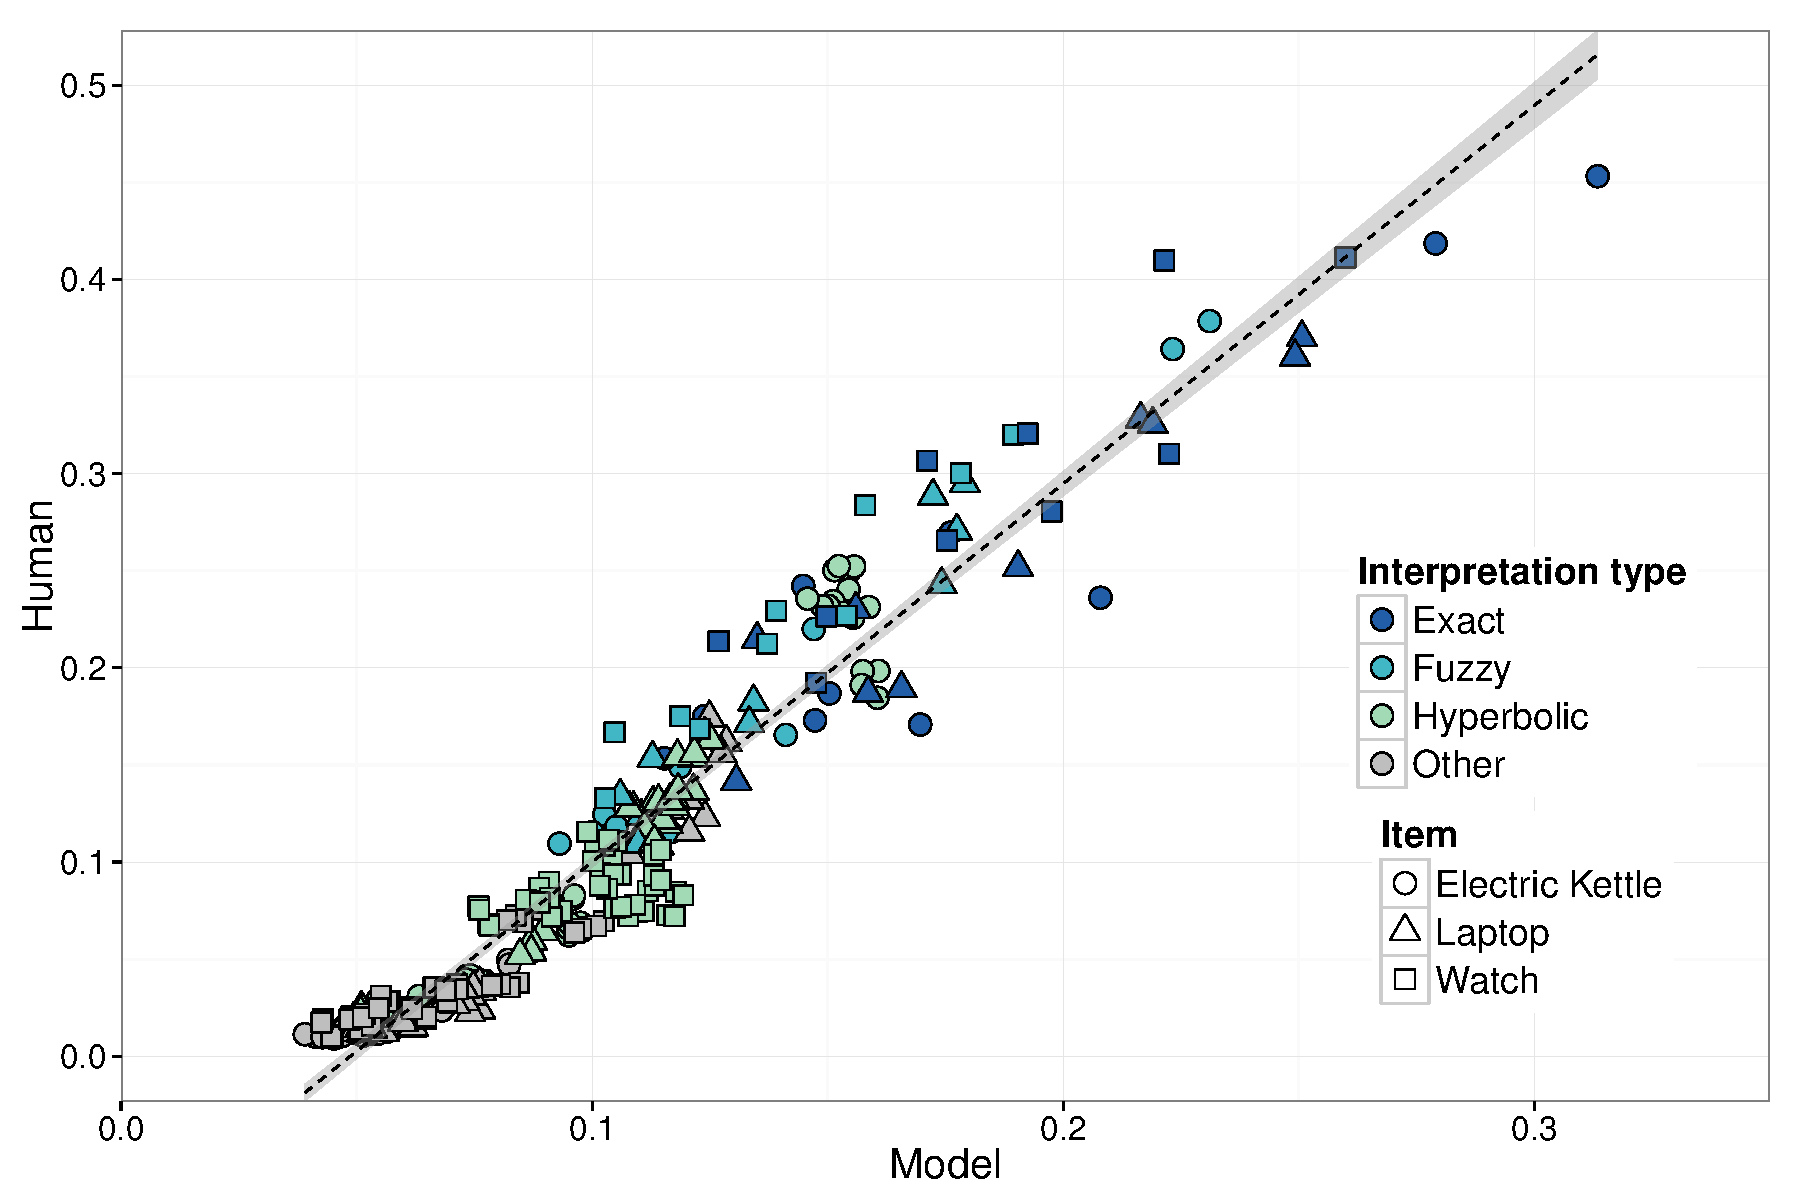
\includegraphics{figure2a-revised.pdf}}
\caption{Model predictions v.s. average human interpretations. Each point represents an utterance and price state pair ($u, s$). The x-coordinate of each point is the probability of the model interpreting utterance $u$ as meaning price state $s$; the y-coordinate is the empirical probability. Correlation between model and human interpretations is $0.968$.}
\label{model_fit}
\end{figure}

\begin{figure}[t]
\centering
\scalebox{0.33}{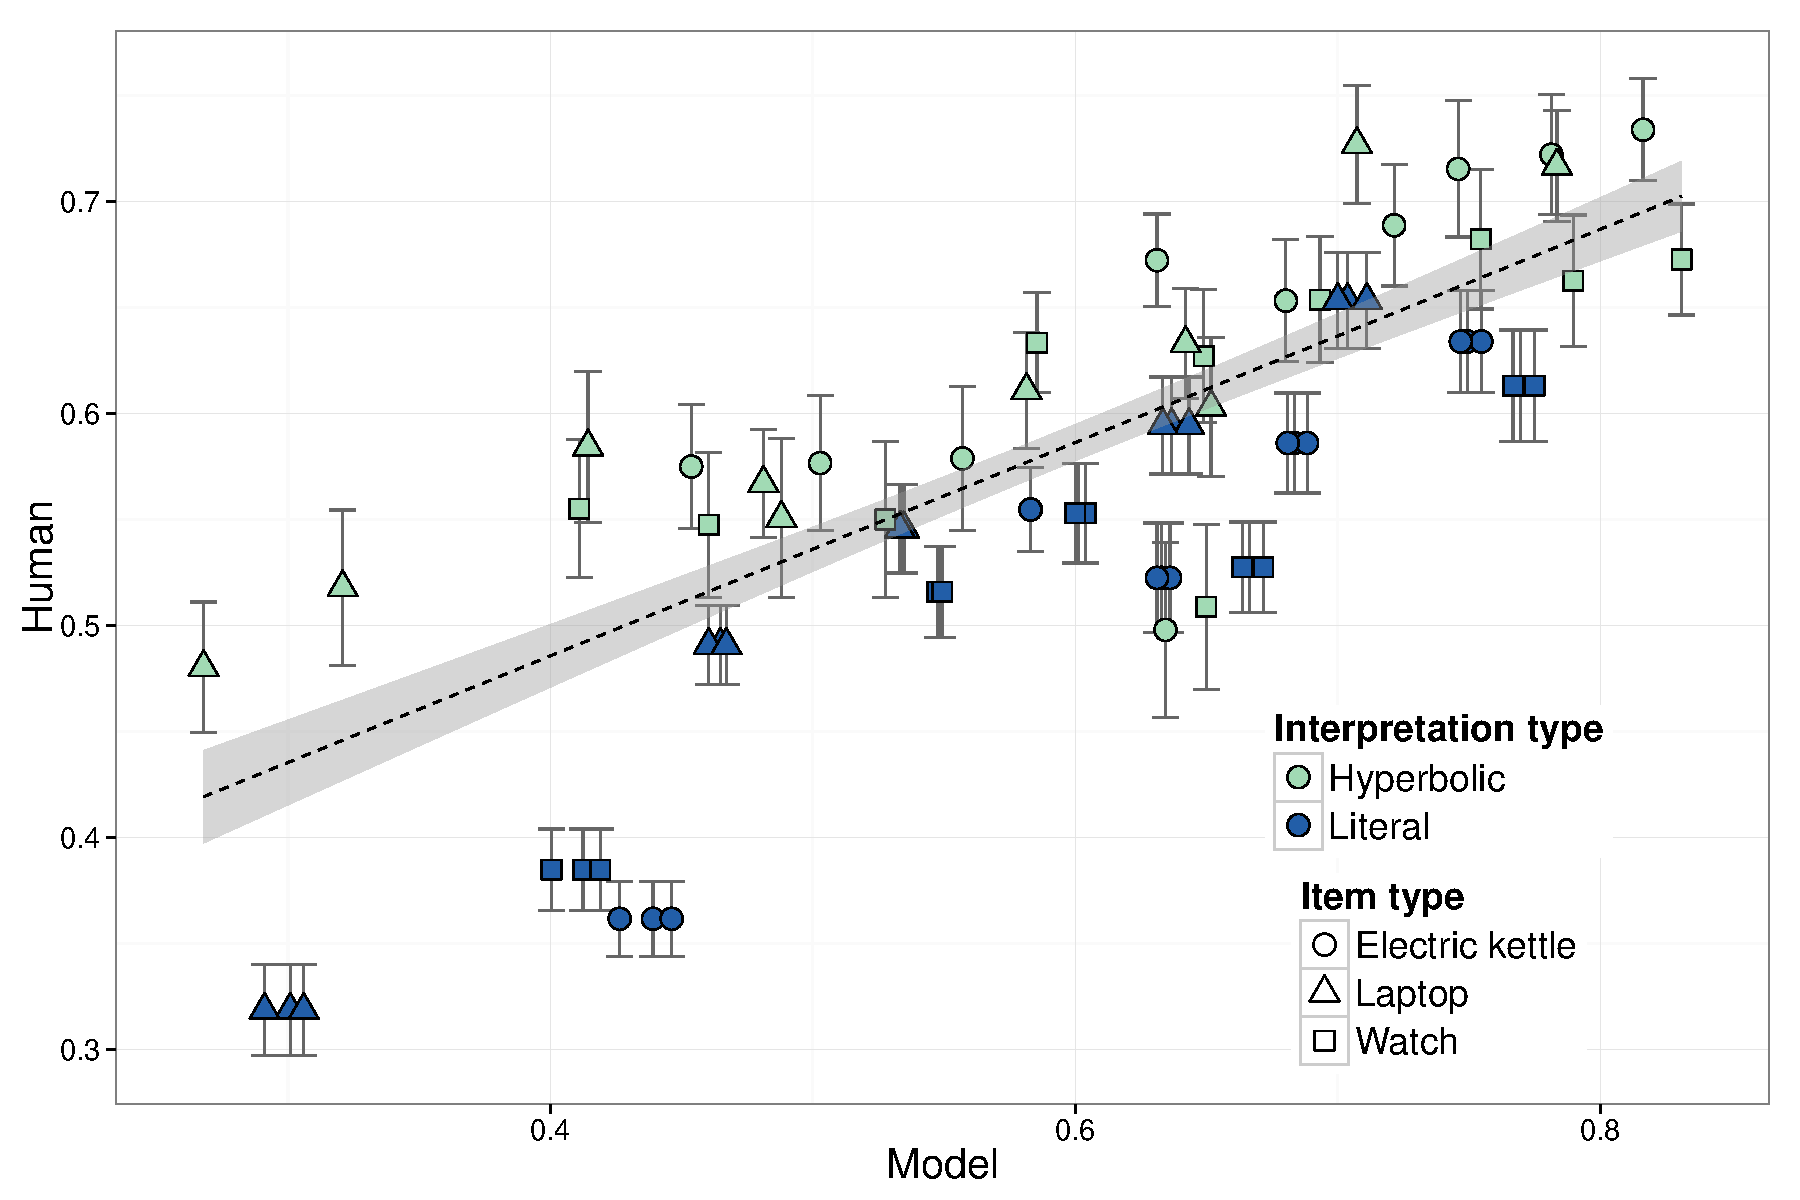
\includegraphics{figure4a-revised.pdf}}
\caption{Model predictions of affect v.s. human ratings. Each point represents an utterance and price state pair $(u, s)$. For pairs where $u = s$, the utterance is literal; for $u > s$, the utterance is hyperbolic. The x-coordinate of each point is the model's prediction of the probability that the utterance/price state pair conveys affect; the y-coordinate is participants' affect ratings (error bars are standard error). Correlation between model and humans is $0.775$.}
\label{affect}
\end{figure}


In \citeA{kao2014figurative}, we examined how people arrive at the appropriate interpretations and affective subtexts of numeric utterances about prices.
%We conducted experiments using the prices of three everyday items---electric kettles, watches, and laptops. 
To empirically measure people's prior beliefs,
we asked participants to rate the probabilities that different items (electric kettles, watches, and laptops) cost various amounts of money (e.g. \$50, \$51, \$1,000, \$10,000). To measure people's encyclopedic knowledge in this domain, we asked participants to rate the probability that someone would think an item that costs \$$x$ is too expensive (e.g., a watch that costs \$1,000). We chose expensiveness as the associated dimension of interest, because utterances about cost seem to naturally evoke judgments of expensiveness \todo{explain this more}.   
Using the empirically measured prior beliefs and background knowledge, we used the qRSA model to obtain predicted interpretations for each utterance. The model reasons about different types of communicative goals that the speaker may have, including the goal to communicate affect about the price of the item. By reasoning about relevance to these communicate goals, the model captures a basic feature of hyperbole: utterances whose literal meanings are less likely given the price prior are more likely to be interpreted hyperbolically. For example, ``The watch cost 1000 dollars'' is more likely to be interpreted hyperbolically than ``The  laptop cost 1000 dollars.'' 

To quantitatively evaluate the model's predictions, we asked participants to interpret potentially hyperbolic utterances. For example, given that Sam said: ``The watch cost 1000 dollars,'' how likely is it that the watch cost $x$ dollars? For all utterances, we then compared the model's and participants' interpretations. The model predictions are highly correlated with people's interpretations ($r=0.968, p<0.0001$) (Figure \ref{model_fit}), suggesting that the qRSA model is able to combine linguistic information, background knowledge, and reasoning about the speaker's goals to interpret hyperbolic utterances. 

%\begin{figure}
%\centering
%\scalebox{0.4}{
%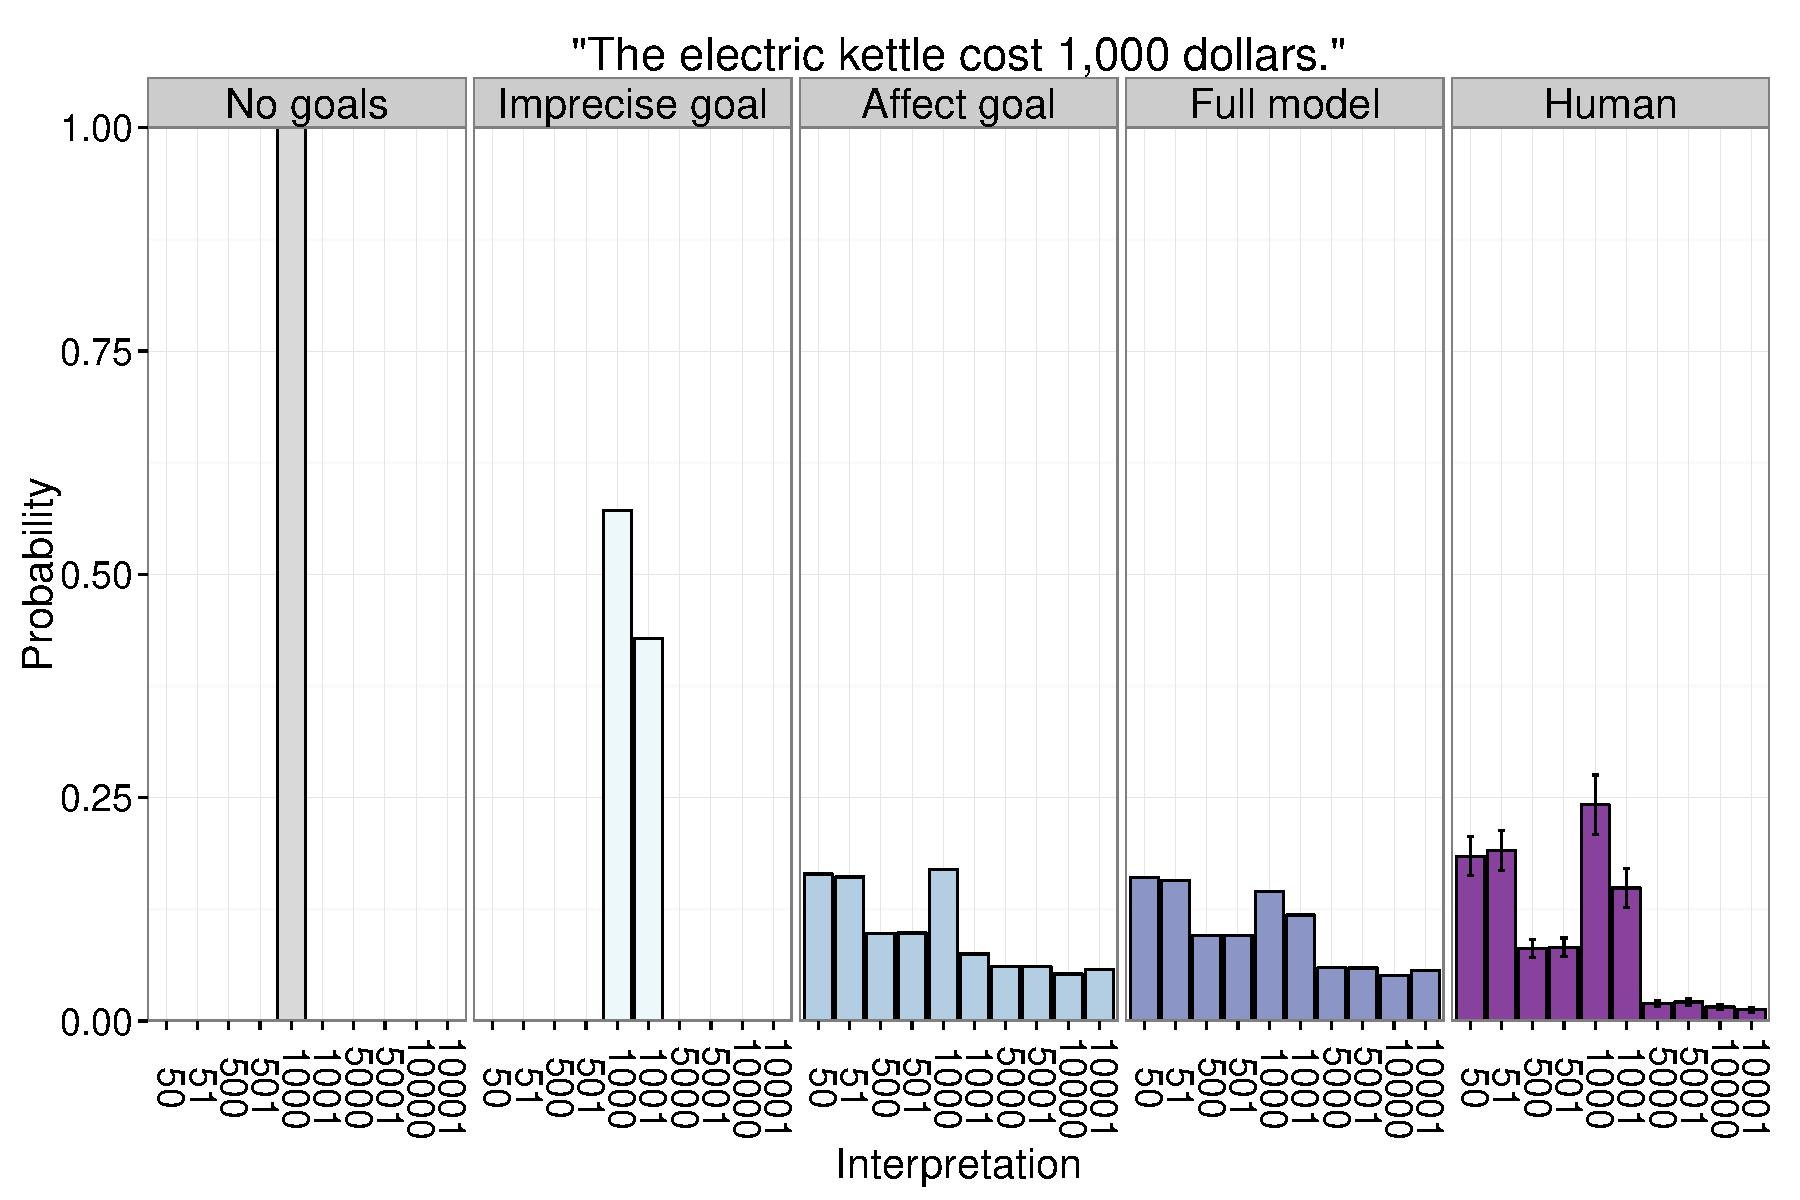
\includegraphics{figure2b-revised.pdf}}
%\caption{Comparison of models with different communicative goals and human interpretations for the utterance ``The electric kettle cost 1,000 dollars.'' A model that considers both affect and precision goals (full model) most closely matches human data.}
%\label{goals}
%\end{figure}

In addition to producing the appropriate corrective response to hyperbolic utterances, the model also captures the affective subtext of hyperbole. We conducted a separate experiment to examine peoples' interpretation of affect in hyperbolic versus literal utterances. Participants read scenarios in which a speaker bought an item that cost $s$ dollars and says it cost $u$ dollars, where $u \geq s$. They then rated how likely it is that the buyer thinks the item was too expensive. Results showed that utterances $u$ where $u > s$ (hyperbolic utterances) are rated as significantly more likely to convey affect than utterances where $u {=} s$ ($F(1, 25)=12.57, p < 0.005$). Moreover, if a watch actually cost $100$ dollars and Sam says something hyperbolic such as ``The watch cost $1000$ dollars,'' people are more likely to believe that Sam thinks the watch is too expensive than if the watch actually cost $1000$ dollars and Sam says ``The watch cost $1000$ dollars.'' This suggests that listeners infer affect from hyperbolic utterances above and beyond the affect associated  with a given price state. Quantitatively, we compared model and human interpretations of affect for each of the 45 utterance and price state pairs $(u, s)$ where $u \geq s$. While there is a significant amount of noise in the human judgments (average split-half correlation is $0.833$), the model predicts human interpretations of the utterances' affective subtext significantly better than chance ($r=0.775, p < 0.00001$), capturing most of the reliable variation in these data (Figure \ref{affect}).
 
Results from \cite{kao2014figurative} suggest that by incorporating inferences about the speaker's communicative goals, the qRSA model successfully interprets hyperbolic utterances and appropriately recovers the affective subtext. 
However, in this initial exploration of applying the qRSA model to figurative language, we only considered a simplified space of affect, namely the presence or absence of negative feeling. 
%This overlooks the range of attitudes and emotions that speakers could express with figurative utterances. 
In the next section, we explore how expanding the space of affect to include emotions with positive/negative valence and high/low arousal accounts for people's interpretations of ironic utterances.
%The model's quantitative predictions closely match humans' judgments on hyperbole, a complex phenomenon previously beyond the scope of computational models.

%\todo[inline]{Propose that the same formal architecture may work for other uses of figurative language that are quite different}
\subsection{Verbal Irony}
%\todo[inline]{Introducing a richer model of affect gives irony}
An ironic statement describes something as contrary to what it actually is \cite{roberts1994people, gibbs1999figurative}. For example, a speaker who says ``Such lovely weather we are having'' in the middle of a storm means that the weather is \emph{not} lovely and expresses a negative attitude towards it. %Like hyperbole, verbal irony also requires the listener to recognize the non-veridicality of the utterance and enter into joint pretense. However, the required corrective response is one of ``kind'' (e.g. from ``lovely'' to ``terrible'') instead of degree (e.g. from ``pouring'' to ``drizzling'') \cite{mccarthy2004there}. 
How do people appropriately interpret these superficially positive or negative utterances? Can our model use QUD inference to interpret an utterance when its literal meaning is not just an exaggerated version of the intended meaning, but rather its opposite?
%\cite{kao2014figurative} showed that this model---which we will refer to as qRSA---produces figurative interpretations of hyperbolic utterances that closely match humans'; however, they considered only a simplified affect space, namely the presence or absence of negative feeling. This overlooks the range of attitudes and emotions that speakers could express with figurative utterances. In particular, since verbal irony involves expressing negative meanings with positive utterances and vice versa, a richer space of affect that includes both positive and negative emotions may be key. 
In this section, we will examine the consequence of expanding the set of emotions we consider to an empirically derived affect space. We show that this minimal change enables the qRSA model to capture many of the rich inferences resulting from verbal irony.

In what follows, we will examine interpretations of potentially ironic utterances in an innocuous domain---the weather. We chose the weather as the victim of irony for several reasons. First, people are quite familiar with talking (and complaining) about the weather. Second, we can visually represent the weather to participants with minimal linguistic description in order to obtain measures of nonlinguistic contextual knowledge. Finally, given the critical role that context plays in understanding irony, we can vary the weather states to observe how the same utterance is interpreted differently given different contextual knowledge. This offers to our knowledge the first fine-grained manipulation and quantitative measure of context in studies of irony. We first explore how an enriched space of affect impacts the qRSA model and find that it produces ironic interpretations in some simple simulations. We then present two behavioral experiments that examine people's interpretations of utterances given different weather contexts. We show that by accounting for two types of affective dimensions, valence and arousal, our model produces interpretations that closely match humans'. 
%Finally, we discuss implications of our model for informal theories of irony and its relationship to other types of figurative language understanding.

\subsubsection{Model}

%In this section, we revisit the qRSA model and compare different spaces of affect to test the conditions for producing ironic interpretations. 

Following the qRSA model described in \cite{kao2014figurative}, a speaker chooses an utterance that most effectively communicates information regarding the question under discussion (QUD) to a literal listener. We consider a meaning space that consists of the variables $s, A$, where $s$ is the state of the world, and $A$ represents the speaker's (potentially multidimensional) affect towards the state. 
We formalize a QUD as a projection from the full meaning space to the subset of interest to the speaker, which could be $s$ or any of the dimensions of $A$. 
We specify the speaker's utility as information gained by the listener about the topic of interest---the negative surprisal of the true state under the listener's distribution given an utterance, $u$, along the QUD dimension, $q$. This leads to the following utility function: 

\begin{equation}
U(u | s, A, q) = \log \sum_{s', A'} \delta_{q(s, A)=q(s', A')} L_{0}(s', A' |u)
\end{equation}
where $L_{0}$ describes the literal listener, who updates her prior beliefs about $s, A$ by assuming the utterance to be true of $s$. 
The speaker $S$ chooses an utterance according to a softmax decision rule \cite{sutton1998reinforcement}:
$S_1(u | s, A, q) \propto e^{\lambda U(u | s, A, q)}$,
where $\lambda$ is the rationality parameter.
%
A pragmatic listener $L_{1}$ then takes into account prior knowledge and his internal model of the speaker to determine the state of the world as well as the speaker's affect. Because $L_{1}$ is uncertain about the QUD, he marginalizes over the possible QUDs under consideration:
$$
L_{1}(s, A | u) \propto P(s) P(A | s) \sum_{q}{P (q) S (u|s, A, q)}
$$
%
The resulting distribution over world states and speaker affects is an interpretation of the utterance. 
\begin{figure}
\centering
\scalebox{0.6}{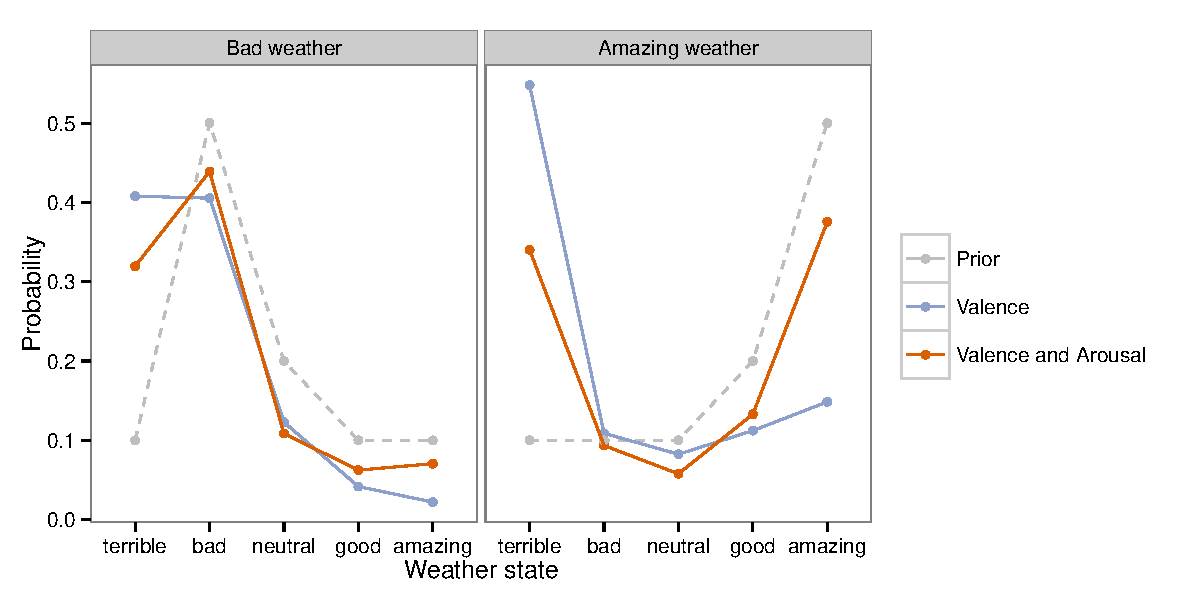
\includegraphics{sim12}}
\caption{Model interpretations of ``The weather is terrible'' given different prior beliefs about the weather state and affect dimensions. Gray dotted lines indicate prior beliefs about weather states given a weather context; blue lines indicate interpretations when reasoning only about the speaker's valence; orange lines indicate interpretations when reasoning about both valence and arousal.}
\label{sim12}
\end{figure}

We performed the following simulations to examine the model's behavior using affect spaces, $A$, that differ in complexity and structure.  
We assume that $s$ has five possible ordered values: \texttt{terrible}, \texttt{bad}, \texttt{neutral}, \texttt{good}, and \texttt{amazing}. We consider two different weather contexts: apparently bad weather and apparently amazing weather, which are each specified by a prior distribution over these states (see gray dotted lines in Figure~\ref{sim12}). We then examine how the model interprets the sentence ``The weather is terrible'' in the two weather contexts, given different affect spaces.

We first consider a one-dimensional affect space, where the dimension is emotional valence, and the values are whether the speaker feels negative or positive valence towards the state.  
The blue lines in Figure~\ref{sim12} show the model's interpretation of ``The weather is terrible'' using this one-dimensional affect space. 
The model is capable of non-literal interpretation: it produces a hyperbolic interpretation (that the weather is merely \texttt{bad}) given ``The weather is terrible'' in the bad weather situation. However, it produces a literal interpretation (that the weather is \texttt{terrible}) in the amazing weather situation. Since a pragmatic listener that only considers emotional valence does not believe that the speaker has any reason to choose a negative utterance to express positive affect (because the utterance communicates no true information), a model that only considers emotional valence is unlikely to infer a positive world state from a negative utterance (and vice versa), thus failing to evidence verbal irony. 

%We now consider a more complex affect space with two dimensions---valence and arousal---to observe its consequence on interpretation. 
What true information \emph{could} a speaker communicate about a positive world state using a negative utterance? Affective science identifies two dimensions, termed valence and arousal, that underly the slew of emotions people experience \cite{russell1980circumplex}. 
For example, \emph{anger} is a negative valence and high arousal emotion, while \emph{contentment} is a positive valence and low arousal emotion. 
%These two dimensions are not independent, with low arousal implying more neutral valence. 
%\todo{JTK: is this non-independence important/necessary to note, or is it confusing?}
%\todo{NDG: is this dependence built into the model's prior? if so, does it matter? if not, we should explore it...} 
Could speakers leverage the arousal dimension to convey high arousal and positive affect (e.g. excitement) using utterances whose literal meanings are associated with high arousal but negative affect (e.g. ``The weather is terrible!'')? We test the consequences of incorporating the arousal dimension. The orange lines in Figure~\ref{sim12} show simulations of the qRSA model with a two-dimensional affect space: whether the speaker feels negative/positive valence and low/high arousal towards the weather state. Given strong prior belief that the weather state is \texttt{bad}, the model interprets ``The weather is terrible'' to mean that the weather is likely to be \texttt{bad}, again producing a hyperbolic interpretation. However, given strong prior belief that the weather is \texttt{amazing}, the model now places much greater probability on the ironical interpretation of ``The weather is terrible,'' meaning that the weather is likely \texttt{amazing}. This is because, with the enriched two-dimensional affect space, the pragmatic listener realizes that the speaker may be using ``terrible'' to communicate high emotional arousal. Note that this result is not simply due to the model falling back on the prior: given the same priors, the model interprets the neutral utterance ``The weather is ok'' as the weather state being \texttt{neutral} and not \texttt{amazing}.
These simulations suggest that a psychologically realistic, two-dimensional affect space enables the qRSA model to interpret ironic utterances in addition to hyperbolic ones. 


%\todo{NDG: perhaps we could have marker size in fig 1 correspond to interpreted arousal? never mind, we don't have that for the first sim...}

\begin{figure*}
    %\centering
    \begin{minipage}{0.45\textwidth}
        %\centering
        \includegraphics[width=220pt, height=150pt]{image-grid}
        \caption{Weather images shown to participants in Experiments 1 and 2.}
        \label{images}
    \end{minipage}
    \hfill
    \hfill
    \begin{minipage}{0.45\textwidth}
       % \centering
        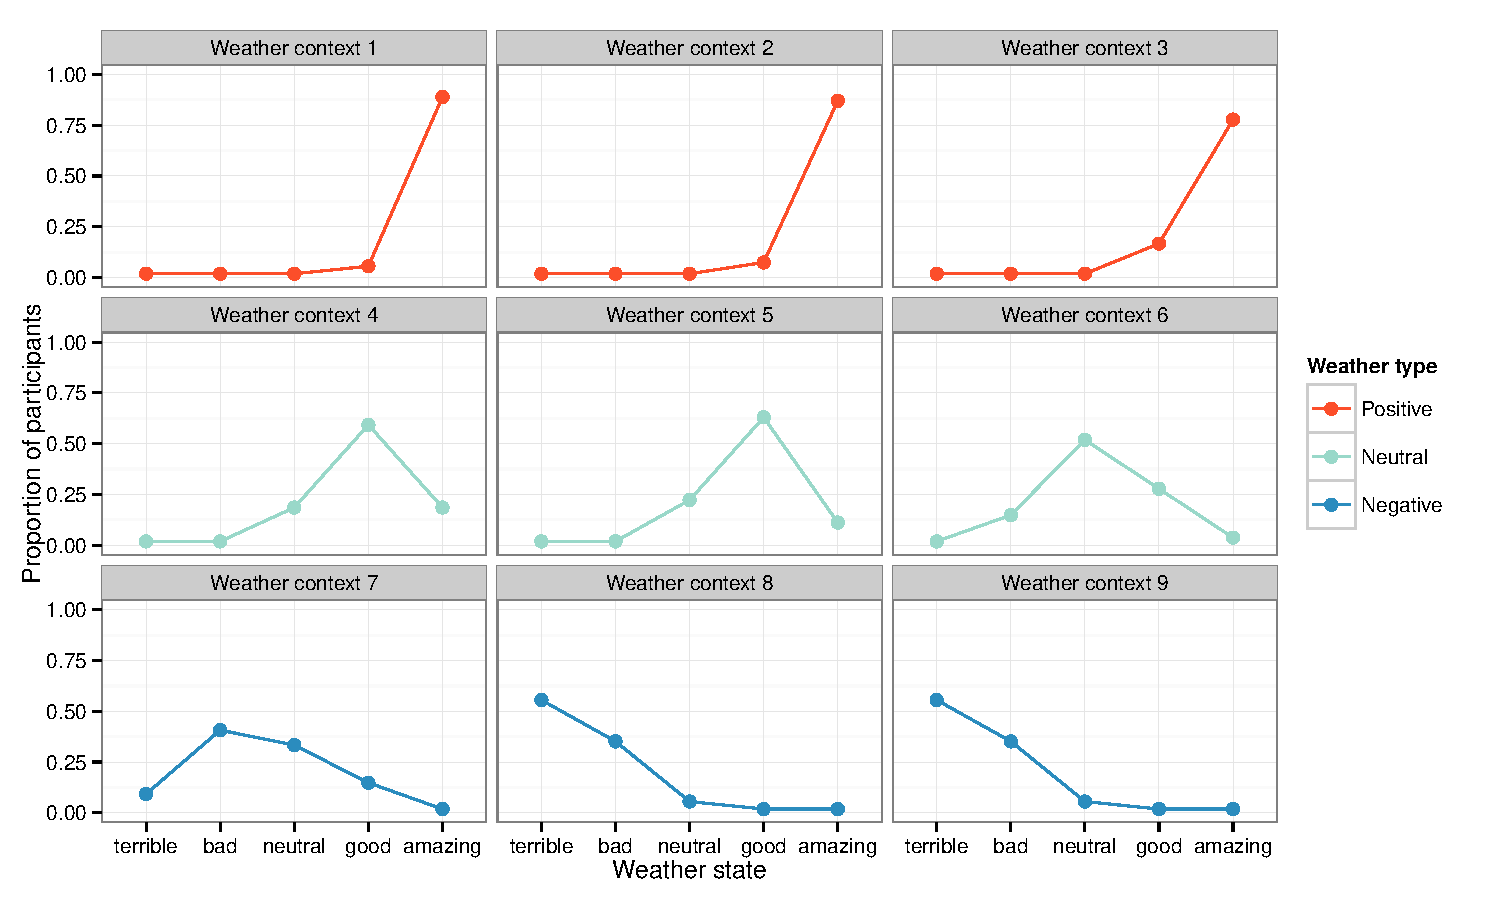
\includegraphics[width=230pt, height=150pt]{priors}
        \caption{Proportion of participants who rated each weather context as each weather state. 
     %Each panel represents a weather context; each line represents the distribution over weather states for a weather context prior to any linguistic input. For example, the vast majority of participants rated weather context 1 as \emph{amazing}, suggesting that the prior probability of someone believing weather context 1 to be \emph{amazing} is extremely high.
     }
        \label{priors}
    \end{minipage}
    %\caption{Nine weather contexts and their empirically measured priors over weather states.}
    %\label{fig:three graphs}
\end{figure*}


\subsubsection{Experiment 1a: Background knowledge for verbal irony}
To quantitatively test whether the qRSA model with expanded affect space can capture a range of ironic interpretations, we need appropriate prior distributions as well as data for human interpretations.
We conducted Experiment 1a to measure prior beliefs over weather states ($P(s)$) for a range of weather contexts as well as the likelihood of various emotions towards each weather state. The latter allows us to empirically derive the affective space and priors, $P(A | s)$, for this domain.
In Experiment 1b, we collected people's ratings of how a speaker perceives and feels about the weather given what she says in a weather context (e.g. ``The weather is terrible!'' when the context clearly depicts sunny weather).
\begin{figure*}
    %\centering
    \begin{minipage}{0.45\textwidth}
        %\centering
        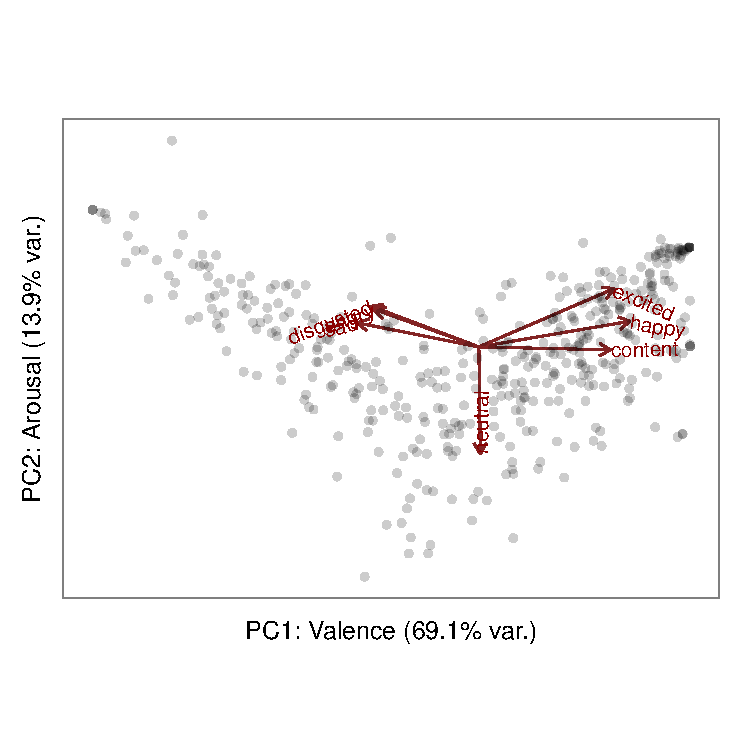
\includegraphics[width=170pt, height=180pt]{biplot.pdf}
        \caption{Biplot of the first two principle components of the seven emotion ratings, which roughly correspond to valence and arousal.}
        \label{pca}
    \end{minipage}
    \hfill
    \hfill
    \begin{minipage}{0.45\textwidth}
       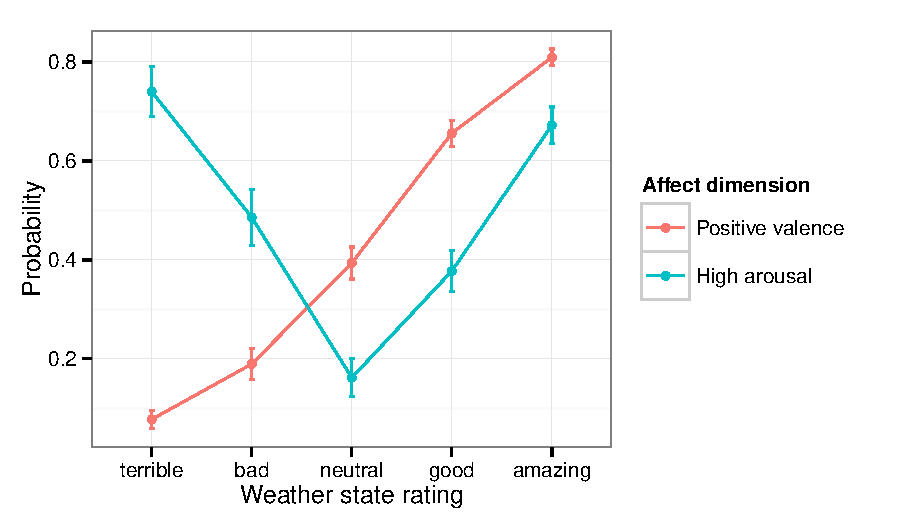
\includegraphics[width=220pt, height=150pt]{affect-prior.pdf}
       \caption{Average probabilities of positive valence and high arousal associated with each weather state; error bars are $95\%$ confidence intervals.}        
        \label{affect-prior}
    \end{minipage}
    %\caption{Nine weather contexts and their empirically measured priors over weather states.}
    %\label{fig:three graphs}
\end{figure*}

%\subsubsection{Experiment 1a: Prior elicitation}
%textbf{Materials and methods}\\
We selected nine images from Google Images that depict the weather. To cover a range of weather states, three of the images were of sunny weather, three of cloudy weather, and three of rainy or snowy weather. We refer to these images as weather contexts. Figure~\ref{images} shows these nine images.
$49$ native English speakers with IP addresses in the United States were recruited on Amazon's Mechanical Turk. Each participant saw all nine images in random order. In each trial, participants were told that a person (e.g.~Ann) looks out the window and sees the view depicted by the image. They then indicated how Ann would rate the weather using a labeled 5-point Likert scale, ranging from \texttt{terrible}, \texttt{bad}, \texttt{neutral}, \texttt{good}, to \texttt{amazing}. Finally, participants used slider bars (end points labeled ``Impossible'' and ``Absolutely certain'') to rate how likely Ann is to feel each of the following seven emotions about the weather: \emph{excited}, \emph{happy}, \emph{content}, \emph{neutral}, \emph{sad}, \emph{disgusted}, and \emph{angry}, which are common emotion categories \cite{ekman1992argument}\footnote{From the most frequently cited set of six basic emotions, we removed \emph{fear} and \emph{surprise} and added \emph{content} and \emph{excited} to have a balanced set of positive and negative emotions. We also added \emph{neutral} to span a wider range of emotional arousal.}.
The order of the emotions was randomized for each participant but remained consistent across trials \footnote{Link to Experiment 1: \url{http://stanford.edu/~justinek/irony_exp/priors/priors.html}}.
\textbf{Results}\\
For each of the nine weather contexts, we obtained the number of participants who gave each of the weather state ratings. By performing add-one Laplace smoothing on the counts, we computed a smoothed prior distribution over weather states given each context, namely $P(s)$ (Figure~\ref{priors}).
% shows that the sunny and positive weather contexts were more likely to be rated as \texttt{amazing}, while the negative weather contexts were more likely to be rated as \texttt{bad} or \texttt{terrible}.  %\todo[inline]{RDH: obviously, need some way of identifying what the different rows and columns of the grid mean}
To examine participants' ratings of the affect associated with each context, we first performed Principal Component Analysis (PCA) on the seven emotion category ratings. This allowed us to compress the ratings onto a lower-dimensional space and reveal the main affective dimensions that are important in this domain, as is often done in affective science \cite{russell1980circumplex}. We found that the first two principal components corresponded to the dimensions of emotional valence and emotional arousal, accounting for $69.14\%$ and $13.86\%$ of the variance in the data, respectively.
%\todo{we should do a free response version of this task (``Ann feels ..... about the weather.''), before and after a statement, at some point to see if we are missing any affects... probably not needed for cogsci.}
The PCA represents emotion ratings for each trial as real values between negative and positive infinity on each of the dimensions. To map these values onto probability space, we first standardized the scores on each dimension to have zero mean and unit variance. We then used the cumulative distribution function to convert the standardized scores into values between $0$ and $1$. 
%\todo{Necessary to say more?} 
This gives us the probabilities of Ann feeling positive (vs.~negative) valence and high (vs.~low) arousal for each trial, which is a two-dimensional probabilistic representation of her affect.
%Although these values are treated as probabilities of a binary variable, they approximately track the \emph{degree} of positive valence and arousal as well; for example, $P(A_v) = 0.6$ suggests that the valence is more positive than neutral, and $P(A_a) = 0.1$ suggests that the arousal is quite low. 
By calculating the average probabilities of positive valence and high arousal given each weather state rating, we obtain the probability of positive valence and high arousal associated with each weather state, namely $P(A | s)$ (Figure ~\ref{affect-prior}).
%\todo[inline]{NDG: does this imply that valence and arousal are independent? they generally aren't.... i'm a bit confused about where the model's $A$ states fall with respect to the valence-arousal quadratic curve....}

%\todo{JTK: something about how this is not a perfect transformation but does approximately the right thing} 

%\begin{figure}
%\begin{minipage}[b]{.5\textwidth}
%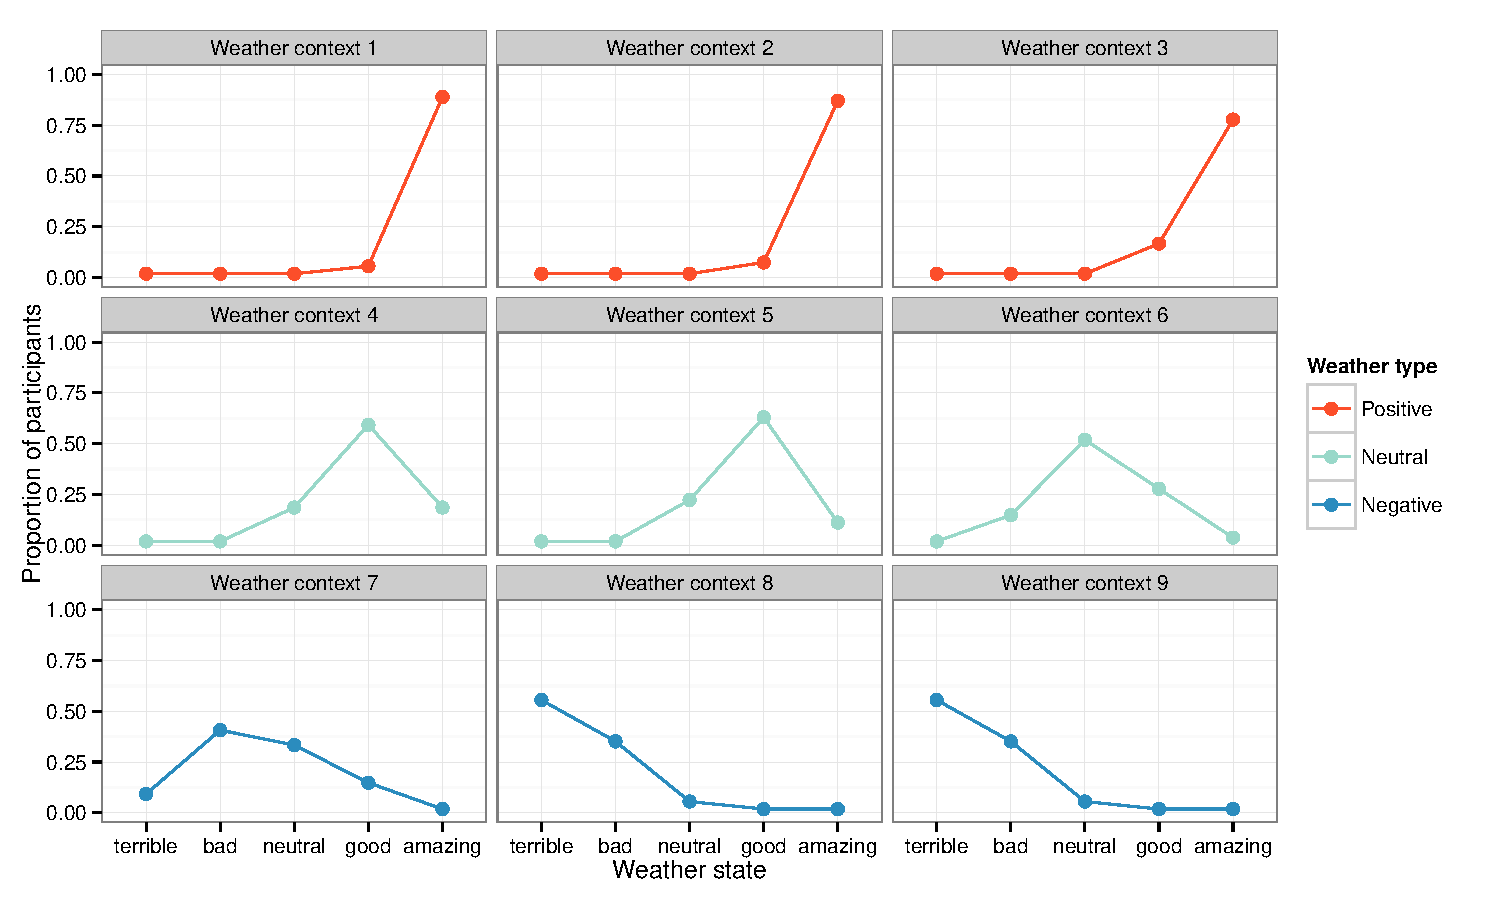
\includegraphics[width=5cm, height=3.7cm]{priors.pdf}
%\end{minipage}
%\begin{minipage}[b]{.4\textwidth}
%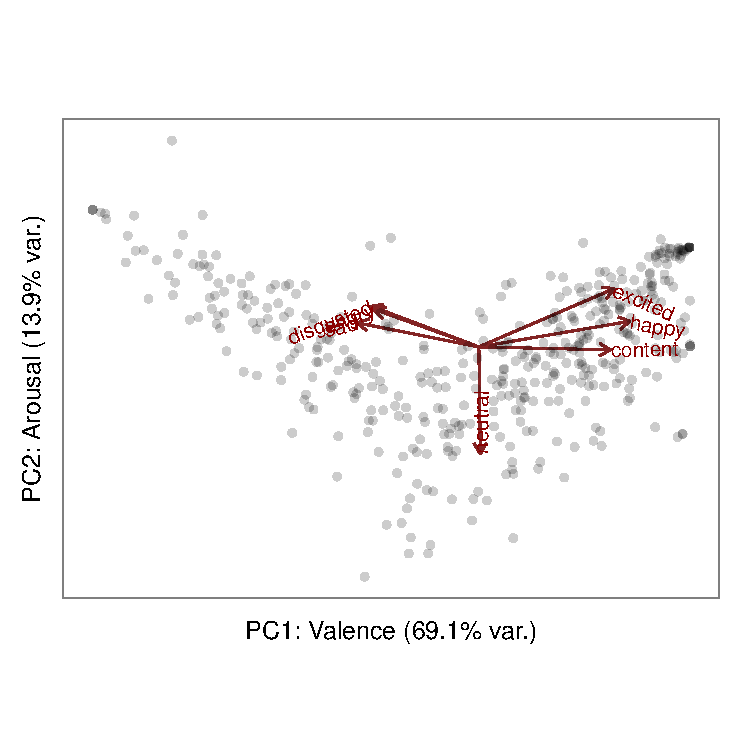
\includegraphics[width=5cm, height=5cm]{biplot.pdf}
%\end{minipage}
%
%\end{figure}

\begin{figure}[t]
\scalebox{0.5}{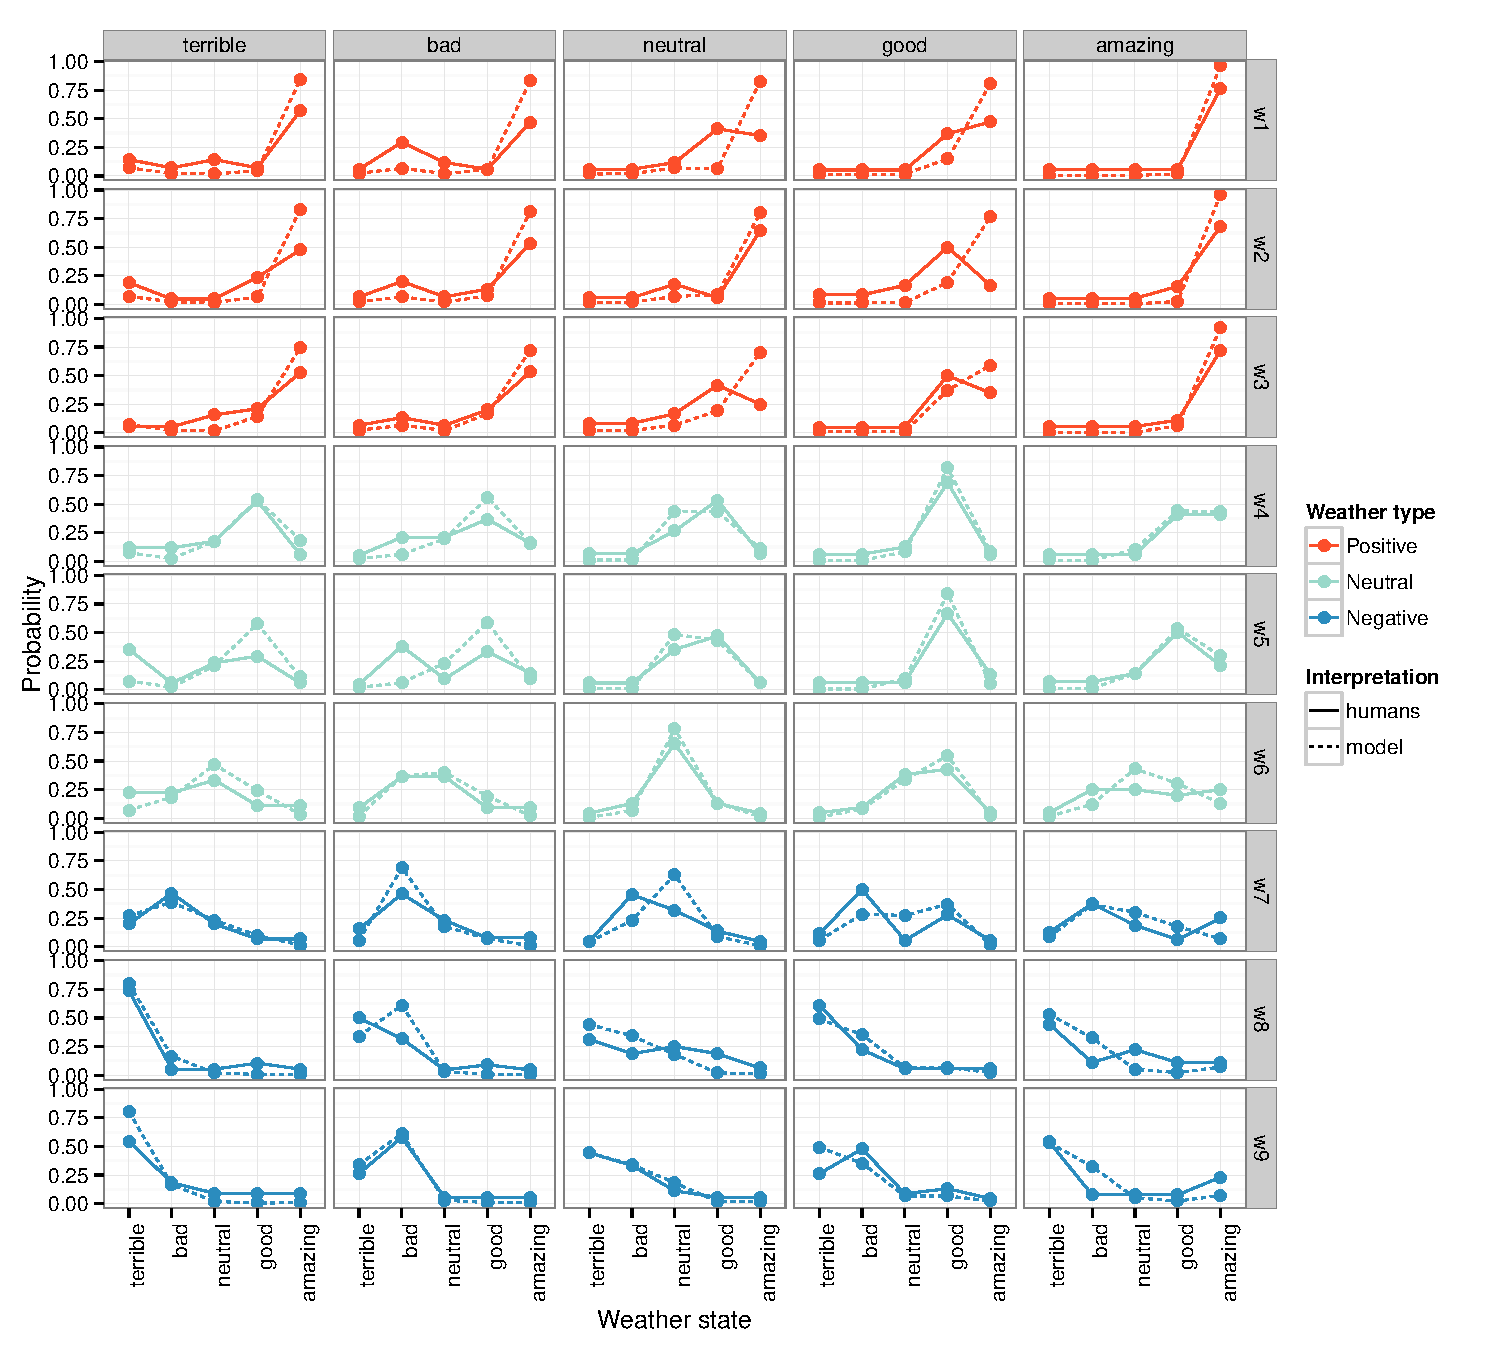
\includegraphics{model-state.pdf}}
\caption{Model's and participants' inferences about the weather state (x-axis) given a weather context (row) and an utterance (column). Each panel represents interpretations of an utterance in a weather context. The solid lines are participants' ratings; the dotted lines are model's posterior distributions over weather states.}
\label{model-state}
\end{figure}


\subsubsection{Experiment 1b: Interpreting verbal irony}
%In Experiment 1, we obtained the prior distribution over weather states for each weather context as well as the prior probabilities of positive valence and high arousal given each weather state. 
Results from Experiment 1b give us the components to generate interpretations of utterances from our model. Here we describe an experiment that elicits people's interpretations of utterances, which we then use to evaluate model predictions. 
%\textbf{Materials and methods}\\

$59$ native English speakers with IP addresses in the United States were recruited on Amazon's Mechanical Turk. Each participant saw all nine images from Figure~\ref{images} in random order. In each trial, participants were told that a person (e.g.~Ann) and her friend are in a room looking out the window together and see the view depicted by the image. Ann says, ``The weather is \underline{\hspace{1cm}}!'' where the adjective is randomly selected at each trial from the following set: ``terrible,'' ``bad,'' ``ok,'' ``good,'' and ``amazing.'' Participants first rated how likely it is that Ann's statement is ironic using a slider with end points labeled ``Definitely NOT ironic'' and ``Definitely ironic.'' They then indicated how Ann would actually rate the weather using a labeled 5-point Likert scale, ranging from \texttt{terrible}, \texttt{bad}, \texttt{neutral}, \texttt{good}, to \texttt{amazing}. Finally, participants used sliders to rate how likely it is that Ann feels each of seven emotions about the weather \footnote{Link to Experiment 2: \url{http://stanford.edu/~justinek/irony_exp/interpretation/interpretation_askIrony.html}}. 

%\textbf{Results}\\
We first examined participants' irony ratings for each of the weather context and utterance pairs. We found a basic irony effect, where utterances whose polarities are inconsistent with the polarity of the weather context are rated as significantly more ironic than utterances whose polarities are consistent with the weather context ($t(34.16)= -11.12, p < 0.0001$). For example, ``The weather is terrible'' (a negative utterance) is rated as more ironic in weather context 1 (positive context) ($M = 0.90$, $SD = 0.21$) than in weather context 7 (negative context) ($M =0.15$,	$SD = 0.27$). A linear regression model with the polarity of the utterance, the polarity of the weather context, and their interaction as predictors of irony ratings produced an adjusted $R^{2}$ of 0.91, capturing most of the variance in the data. This suggests that participants' lay judgments of irony align with its basic definition: utterances whose apparent meanings are opposite in polarity to the speaker's intended meaning.
Given the fact that participants can identify verbal irony based on its inconsistency with context, how do they then use context to determine the speaker's intended meaning? We examined participants' interpretations of utterances given contexts. For each of the $45$ weather context (9) $\times$ utterance (5) pairs, we obtained the number of participants who gave each of the five weather state ratings (\texttt{terrible, bad, neutral, good, amazing}). We performed add-one Laplace smoothing on the counts to obtain a smoothed distribution over weather states given each context and utterance (solid lines in Figure~\ref{model-state}). Results show that participants produce ironic interpretations of utterances, such that the weather is most likely to be \texttt{amazing} given that the speaker said ``The weather is terrible'' in weather context 1. Participants also produce hyperbolic interpretations, such that the weather is most likely to be \texttt{bad} given that the speaker said ``The weather is terrible'' in weather context 7. This confirms the intuition that people are highly sensitive to context and use it both to determine when an utterance is not meant literally and to appropriately recover the intended meaning. 
%
Finally, we examine participants' inferences about the speaker's affect given utterances in context. We used the loadings from the PCA on emotion ratings from Experiment 1 to project the emotion ratings from Experiment 2 onto the same dimensions. We then standardized and converted the scores into values between $0$ and $1$, as before, which gives us probability ratings of the speaker feeling positive valence and high arousal given an utterance and weather context.
%Figure ~\ref{valence} shows the average probability of \emph{positive valence} given an utterance in a weather context. The dotted gray lines are the average probabilities of positive valence associated with each weather context without any linguistic input, taken from Experiment 1. 
%
%We see that for the \emph{positive} weather contexts, the speaker is interpreted as more likely expressing positive valence given the extremely negative utterance ``terrible'' than given the less negative utterance ``bad.'' On the other hand, for the \emph{negative} weather contexts, the speaker is interpreted as less likely expressing positive valence given the extremely positive utterance ``amazing'' than the less positive utterance ``good'' (STATS). This suggests that extreme utterances that are inconsistent with the valence of the context are more likely to express an opposite affect than its literal meaning.
%\todo[inline]{maybe you could use different names for the weather contexts? Like $\mathcal{W}_{neg}, \mathcal{W}_{neut}, \mathcal{W}_{pos}$, and then refer to $w_i \in \mathcal{W}_{neg}$ and so on.}
%
%Figure ~\ref{arousal} shows the average probability of \emph{high arousal} given an utterance in a weather context. The dotted gray lines are the average probabilities of high arousal associated with each weather context without any linguistic input, taken from Experiment 1. 
%We see that regardless of the weather context, more extreme utterances (e.g. ``terrible'' and ``amazing'') are more likely to communicate high arousal.
%\todo[inline]{JTK: figure out data take-home point here}
%\todo{it's interesting that ``terrible'' seems to have suppressed arousal compared to ``bad''. any thoughts about why?}


%We call this distribution the \emph{interpreted meaning} of an utterance in context. We found that participants often rated the speaker (e.g. Ann) as judging the actual weather state to be different from what she described in her utterance, suggesting that participants interpreted these utterances non-literally. To further examine the relationship between literal meaning, interpreted meaning, and judgements of irony, we computed the Kullback-Leibler divergence between the literal interpretation of the utterance and the distribution over weather states given the context and utterance. 
%\todo{what is the literal distribution? if it's delta on the word corresponding state, then isn't KL just the interpretation log-prob of the state?}
%\todo[inline]{RDH: I don't quite understand what the KL divergence is measuring in the next paragraph}
%
%We found that adding the KL divergence measure to the linear regression model captured significantly more variance in the irony ratings, with an R-squared of 0.93 (more STATS). 
%\todo{this doesn't seem like the right analysis.... and a 1\% gain is pretty minimal to fuss about.} 
\begin{figure}[t]
\centering
%\begin{subfigure}{0.7\textwidth}
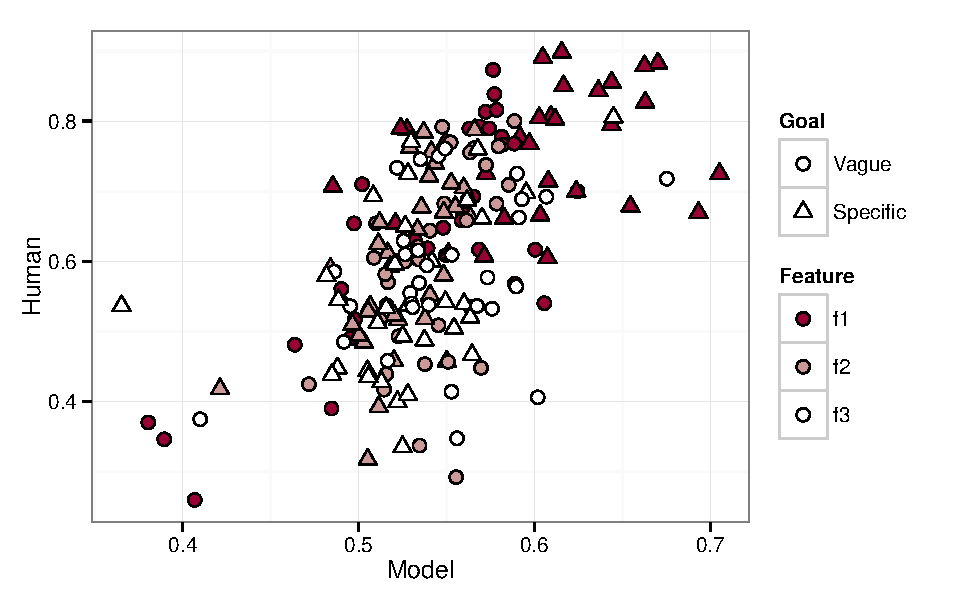
\includegraphics[width=340pt, height=170pt]{scatter.pdf}
\caption{Scatter plot showing correlations between model predictions and human ratings for weather state, speaker valence, and speaker affect. Colors indicate utterances.}
\label{scatter}
%\end{subfigure}
%\begin{subfigure}{0.43\textwidth}
%\includegraphics[width=220pt, height=140pt]{model-arousal.pdf}
%\caption{Average probabilities of speaker feeling high arousal given her utterance in a weather context.}
%\label{arousal}
%\end{subfigure}
%\begin{subfigure}{0.15\textwidth}
%\includegraphics[width=75pt, height=140pt]{scatters.pdf}
%\caption{Scatter plot of human versus model interpretations.}
%\label{scatter}
%\end{subfigure}
\end{figure}

\subsubsection{Irony model evaluation}
From Experiment 1a, we obtained the prior probability of a weather state given a context ($P(s)$) as well as the probability of affect given a weather state ($P(A | s)$). In addition, we fit three free parameters to maximize correlation with data from Experiment 1b: the speaker optimality parameter ($\lambda = 1)$ and the prior probability of each of the three QUDs ($P(q_{state}) = 0.3$, $P(q_{valence}) = 0.3$, $P(q_{arousal}) = 0.4$)\footnote{Since $P(q_{state}) + P(q_{valence}) + P(q_{arousal}) = 1$, $P(q_{arousal})$ is determined by the other two QUD parameters and not a free parameter.}.
%\todo{NDG: the three QUD probs aren't independent, so only 3 free params, right?}  
For each of the $45$ utterance and weather context pairs, the model produced an interpretation consisting of the joint posterior distribution $P(s, A | u)$, where $A$ can be further broken down into valence and arousal dimensions. We will examine the model's performance on each of these state and affect dimensions by marginalizing over the other dimensions.

%\todo[inline]{NDG: for each of these correlations also report percent of explainable variance captured with CI (footnote can explain what that is) JTK: still need to do this.}
Figure ~\ref{scatter} shows scatter plots correlating model predictions with human interpretation data for each of the dimensions: weather state, valence, and arousal. %Figure ~\ref{model-state} shows participants' and the model's inferences about the actual weather state given an utterance and a weather context. 
The model predictions of weather state given utterance match humans' interpretations, with a correlation of $0.86$. Since the split-half correlation for the human data is $\rho=0.898$ ($95\%$CI $= [0.892, 0.903]$)\footnote{Split-half correlations $\rho$ were calculated by repeatedly bootstrapping samples from the data (sample each participant with replacement), computing correlation between two halves of the bootstrapped samples, and using the Spearman-Brown prediction formula to estimate predicted reliability with full sample size. Confidence intervals are $95\%$ CI over $1000$ iterations of bootstrap sampling.\label{splithalf}}  we find that our model captures much of the explainable variance in human judgements. The model predicts humans' interpretations of valence extremely well, with a correlation of $0.96$, capturing essentially all of the explainable variance in the data ($\rho = 0.948\pm0.001$).
%Figure ~\ref{valence} shows participants' and the models' inference about the speaker's valence given an utterance and a weather context. From the tight correspondence between model and human interpretations of valence ($r=0.96$), we see that the model is able to incorporate the valence associated with the utterance's literal meaning (e.g. ``The weather is terrible'') and the valence associated with the weather context (e.g. weather context 1) to interpret the probability of the speaker feeling positive valence. 
Importantly, the model infers the appropriate valence even when it is inconsistent with the valence of the utterance's literal meaning. 
%\todo{note that this is the case even when interpreted valence mismatches the prior expected valence given literal meaning -- i.e. the model captures irony in valence.}
The model's predictions for emotional arousal match humans' with a correlation of $0.66$, capturing a substantial amount of the explainable variance ($\rho = 0.763\pm0.005$). Furthermore, the absolute difference between the model's inferred valence and the valence of the utterance's literal meaning correlates significantly with people's irony ratings ($r = 0.86$, $\rho=0.94 \pm 0.005$), suggesting that the model is able to use inconsistencies between literal and interpreted meanings to identify ironic uses.
%\todo[inline]{JTK: still need to do stats for this}
%Figure~\ref{arousal} shows participants' and the model's inferences about the speaker's arousal. 
%\todo{why is this correlation low? is it because of the terrible-bad inversion i asked about above?}

\begin{table}
\centering
\begin{tabular}{ |c | c | c | c | c | }
  \hline
  \textbf{Model} & \textbf{State} & \textbf{Valence} & \textbf{Arousal} & \textbf{Average} \\\hline                        
  Literal & 0.38 & 0.45 & 0.49 & 0.44\\
  Prior & 0.79 & 0.84 & 0.49 &  0.71 \\
  Valence & 0.84 & 0.79 & 0.61 & 0.75 \\
  Valence + arousal & 0.86 & 0.96 & 0.66 & 0.83\\
  \hline 
  Best possible & 0.90 & 0.95 & 0.76 & 0.87\\\hline
\end{tabular}
\caption{Correlation coefficients between model predictions and human interpretations of weather state, valence, and arousal given an utterance and weather context from Experiment 2. \emph{Best possible} gives an estimate of the maximum possible correlation given noise in the data (see footnote \ref{splithalf}).}
\label{table1}
\end{table}

We considered a series of simpler models to show that the full model using a two-dimensional affect space best predicts human interpretations. 
%\todo{JTK:Should I add a line for split-half in table?}
We first examined a model that interprets utterances literally, such that ``The weather is terrible'' is always interpreted as the weather state being \texttt{terrible}, along with the valence and arousal associated with \texttt{terrible} weather. 
%Such a model produces a distribution over states that correlates with humans' interpretations with $r=0.38$, inference about valence that correlates with humans' with $r=0.45$, and inferences about arousal with a correlation of $r=0.49$. 
We then examined a model that simply ignores the speaker's utterance and takes into account only the state and affect priors associated with each weather context. 
%Such a model produces a distribution over states that correlates with humans' interpretations with $r=0.79$, inferences abut valence that correlate with $r=0.84$, and inferences about arousal that correlate with $r= 0.49$. 
Finally, we examined the performance of the qRSA model with a unidimensional affect space (valence only). 
Table~\ref{table1} shows the models' correlations with human judgements for state, valence, and affect.
A complete model that takes into account prior knowledge, the literal meaning of the utterance, and a two-dimensional affect space outperforms the other models. This dominance is especially apparent with respect to inferences about valence, which is the most important aspect of understanding an ironic utterance, since the listener must infer the intended positive/negative valence from an ostensibly negative/positive utterance. These comparisons suggest that our full model successfully leverages richer knowledge of affect and uses pragmatic reasoning to produce the appropriate figurative interpretations.
%, both ironic and hyperbolic. 
%Fitting two free parameters to maximize fit with human data, the model obtains a state correlation of $r=0.84$, a valence correlation of $r=0.79$, and an arousal correlation of $r=0.61$.


%\todo[inline]{it would be nice to have some more direct analysis of irony -- that when state/valence mismatches that expected from literal meaning the model can predict it. this may also be a good place to come back to the explicit irony judgements: something like probability the interpretation is on the opposite side of the prior mean? or something more general that would also apply to ironic propositions? oh.. we should totally say something in the discussion about ironic propositions and other non-scalar irony.}

\subsubsection{Discussion}
%\todo[inline]{Add something about common ground and in-group?}
%\todo[inline]{summary of take-home point}
In this work, we formalized intuitions about verbal irony understanding and clarified the role of shared prior knowledge in ironic interpretations. We explored the consequences of expanding the space of affect considered by previous Rational Speech Act models to account for verbal irony. By making a minimal extension to \cite{kao2014figurative}'s hyperbole model, we were able to capture people's fine-grained interpretations of ironic utterances in addition to hyperbole. This provides evidence that hyperbole and irony may operate using similar underlying principles of communication---reasoning about shared background knowledge as well as the speaker's affective goals.
%, which are not immediately predictable from the literal semantics of an utterance. 
%By providing fine-grained and quantitative manipulations of shared prior knowledge, we may begin to examine why using irony highlights common ground and group membership \cite{gibbs2000irony}.

%The novelty of the paper is to present a way of quantifying the prior expectations and clarifying their role in rational inferences to derive an interpretation that is not at all predictable given the semantically encoded information.
%, which aligns with other informal accounts of the pragmatics of figurative language understanding (cite).  

%There remain important qualities of verbal irony to account for. For example, speakers often use verbal irony to remind the listener of previous utterances that turned out to be false, or of positive norms that were violated \cite{sperber1981irony, jorgensen1984test}. On the other hand, pretense theory argues that when a speaker produces an ironic utterance, she is only pretending to be someone who would make such an utterance \cite{clark1984pretense}. 
%In this view, recognizing the pretense is central to interpreting verbal irony.
%The latter point in particular has interesting implications on the experiments we present here. While we asked participants to rate the speaker's affect given her utterance, it may be the case that the speaker is only \emph{pretending} to  
%\todo{JTK: Say something about how terrible may involve pretense?} 
%While our model is able to capture the main characteristics of verbal irony, it does not account for the intuitions behind echoic mention or pretense theories. We hope to enrich our model's understanding of the social aspects of irony by addressing these intuitions in future research. In addition, we aim to further examine how people identify the particular dimensions of meaning that may be under discussion in a given context. For example, affective dimensions such as valence and arousal may be particularly relevant in domains that involve evaluation (e.g. ``good'' or ``terrible'' weather), while non-affective dimensions may be more salient in other domains \cite{kao2014formalizing}.
%\todo[inline]{JTK: say something about non-scalar irony?}

%\todo{JTK: Is this paragraph necessary? Should we instead talk more about future research regarding common ground manipulations and other kinds of affect?}
%Beyond shedding light on the communicative principles underlying irony understanding, our work also has interesting connections to natural language processing. Many researchers aim to automatically detect sarcasm in order to recover the correct sentiment from large bodies of text. %(e.g. ``I was overjoyed to pay $\$30$ for an overcooked steak'') 
%\cite{davidov2010semi, filatova2012irony}. %
%By integrating background knowledge and linguistic meaning in a principled manner, our model provides a deeper understanding of context and common ground that most NLP approaches currently lack \cite{gonzalez2011identifying, wallacehumans}.


%Overall, our experimental paradigm and modeling framework provide a detailed and precise account of irony understanding. Given the prevalence of irony in everyday language and the social functions it serves, we believe it would be \emph{amazing} to understand how people interpret utterances that convey the opposite of what they ostensibly mean ($\#$notsarcastic). 

\subsection{Metaphor}
%\todo[inline]{first review discourse goals; then list and characteristics of metaphor} 
%\todo[inline]{hyperbolic/strikingness (compare with literal utterance); aptness; efficiency}
%\todo[inline]{one study/model for studying each characteristics}
%\todo[inline]{Basic: how the model gets basic metaphorical/figurative interpretation of scalar metaphors}
%\todo[inline]{Compared to literal alternatives, metaphors are more striking/extreme}
%\todo[inline]{Compared to other metaphorical alternatives, some metaphors are better/more apt}
%\todo[inline]{Metaphors communicate more efficiently. Look at feature metaphors}

Metaphors are utterances that implicitly compare ideas or concepts from different domains \cite{gibbs1999figurative, roberts1994people}. 
%For example, ``Juliet is the sun'' expresses Juliet's beauty; ``My lawyer is a shark'' communicates the lawyer's ruthlessness; and ``Art washes away from the soul the dust of everyday life'' allows Picasso to compare ``art'' to a cleansing fluid and ``the soul'' to a physical object that collects dust, which gracefully accomplishes two poetic metaphors at once. One can find traces of metaphoricity even in mundane utterances such as ``I waited for a long time,'' where the spatial term ``long'' is used to describe the abstract domain of time \cite{lakoff1993contemporary}. Due in part to its ubiquity and in part to the possibility that metaphor is intimately tied to our ability to create mappings between concrete experiences and abstract concepts \cite{lakoff2008metaphors}, metaphor is by far the most widely studied trope in cognitive science and related fields \cite{gibbs2012interpreting}.
It has inspired a particularly impressive amount of research in cognitive science, spanning topics such as how metaphors structure and shape our thoughts \cite{ortony1993metaphor, lakoff1993contemporary, thibodeau2011metaphors}, whether metaphor processing recruits the same strategies as standard language processing \cite{giora1997understanding, gibbs2002new, glucksberg1993metaphors} and what factors determine people's interpretation a novel metaphor \cite{gentner1997alignment, blasko1993effects, tourangeau1981aptness, kintsch2002metaphor}. This overwhelming interest in metaphor research is due to both the ubiquity of metaphor in everyday language and the potential role of metaphor for helping us understand how the mind creates meaning.

Why do people choose to use metaphors to communicate? What are some characteristics of metaphor that contribute to its popularity? \citeA{roberts1994people} examined the discourse goals that people have when they use various figurative tropes. They found that the most common goals for using metaphor were to clarify ($82\%$), to add interest ($71\%$), to compare similarities ($35\%$), to provoke thought ($35\%$), and to be eloquent ($35\%$). Interestingly, although metaphors are defined as implicit comparisons, ``to compare similarities'' is less frequently listed as a goal than ``to clarify'' and ``to add interest.'' This suggests that beyond examining the cognitive processes for comparing and aligning concepts that may be involved in metaphor understanding, it is also important to consider other higher-level communicative functions that metaphors may serve.

%\subsubsection{Subjective attitude}
%Although emotion goals were not listed among the popular discourse goals for metaphor in \cite{roberts1994people}, other researchers have suggested that metaphors are often used to express subjective attitudes towards the subject \cite{ortony1979beyond}. \citeA{riloff2005exploiting} noted that subjective sentences frequently contain figures of speech such as metaphor and hyperbole. Since metaphor describes an ``experienced'' reality rather than actual reality \cite{ortony1975metaphors}, it is perhaps inherently subjective.  By using metaphorical language, speakers may be signaling to the listener that the information conveyed is a product of the speaker's subjective evaluation and not the objective truth.

%\subsubsection{Efficiency}
In addition to \cite{roberts1994people}'s exploration of discourse goals, other researchers have suggested that metaphorical utterances can be used to efficiently express complex meanings  \cite{ortony1975metaphors, boerger2005variations,glucksberg1989metaphors}. In communication tasks where pairs of participants are separated by a screen and asked to refer to abstract geometrical objects, participants often prefer to describe objects analogically in terms of other known objects rather than use literal analytical descriptions \cite{clark1986referring, glucksberg1989metaphors}. \citeA{fussell1989effects} found that these analogical and figurative descriptions tend to be shorter than literal descriptions. In addition, they found that figurative descriptions are used significantly more often when the intended audience is one's self, where presumably there is a great deal of common ground, than when the intended audience is a different person. These findings suggest that people may be balancing efficiency and clarity when choosing figurative versus literal descriptions. \cite{glucksberg1990understanding} wrote, ``Metaphors are  used  to  communicate a complex, patterned  set of properties in a shorthand that is understood  by the  members of a speech community  who share relevant mutual  knowledge'' (pp. 16). As a result, a potential benefit of speaking in metaphor may be to utilize common ground to communicate both clearly and efficiently. 
%

In my dissertation, I plan to examine the following (hypothesized) characteristics of metaphorical utterances: (1) metaphors lead to more striking, or extreme, interpretations than literal descriptions (2) metaphors can communicate information along various dimensions with a minimal number of words (3) the interpretation of a metaphor is highly sensitive to the local context (4) the aptness of a metaphor is related to whether there are alternative utterances that can communicate the same amount of information more efficiently.
To examine these hypotheses, I will test the qRSA model on different types of metaphorical interpretations.

\subsection{Model sketch}
%In our formalization, a listener assumes that the speaker chooses an utterance to maximize informativeness about a subject along dimensions that are relevant to the QUD and consistent with the speaker's communicative goal. 
To reasonably limit the scope of our work, we focus on metaphors of the classic form ``$X$ is a $Y$.'' Suppose a speaker uses the following utterance to describe a person, Bob: ``Bob is a giraffe.'' How should a listener interpret this utterance?
Following the qRSA framework, a listener again assumes that the speaker chooses an utterance to maximize informativeness about a subject along dimensions that are relevant to the QUD. Unlike hyperbole and irony, however, these dimensions are not affective in nature. Rather, they are features associated with the metaphorical source, in this case ``giraffe.''

We again introduce a literal listener $L_0$, who interprets the utterances as meaning that Bob is literally a giraffe. Since $L_0$ believes Bob is a giraffe, she also believes that Bob is likely to have features associated with giraffes, for example, being tall.
The following equation represents the literal listener's interpretation, where $c$ is Bob's category (either a ``person'' or a ``giraffe''), and $\vec f$ is a vector representation of Bob's features. $P(\vec f | c)$ is thus the prior probability that a member of category $c$ has feature vector $\vec f$.

\[ L_0(c, \vec f |u) = \left\{ 
  \begin{array}{l l}
    P(\vec f | c) & \quad \text{if $c$ = $u$}\\
    0 & \quad \text{otherwise}
  \end{array} \right.\]
%and conduct behavioral experiments to evaluate the model's performance. We show that peoples' interpretations of metaphors are driven by conversational context and that our model captures this effect. Finally, we show that our model predictions correlate significantly with people's fine-grained interpretations of metaphorical utterances.
%
The QUD may be Bob's species category, or Bob's feature(s). We define the speaker's utility as the negative surprisal of the true state under the listener's distribution, projected along the QUD dimension. This leads to the following utility function for speaker $S_1$:
\begin{equation}
U(u | Q, c, \vec f) = \log \sum_{c,\vec f} \delta_{Q(c, \vec f)=Q(c', \vec f')} L_0(c', \vec f' |u)
\end{equation}
Given this utility function, the speaker chooses an utterance according to a softmax decision rule that describes an approximately rational planner \cite{sutton1998reinforcement}, where $\lambda$ is an optimality parameter:
\begin{equation}
S_1(u | Q, c, \vec f) \propto e^{\lambda U(u | Q, c, \vec f)},
\end{equation}
%
The pragmatic listener $L_1$ uses Bayesian inference to guess the intended meaning given prior knowledge and his internal model of the speaker. To determine the speaker's intended meaning, $L_1$ marginalizes over the possible speaker goals under consideration:
$$
L_1 (c, \vec f | u) \propto P(c) P(\vec f | c) \sum_{Q}{P (Q) S_1 (u|Q, c, \vec f)}
$$

If $L_1$ believes it is \emph{a priori} very unlikely that Bob is actually a giraffe and that $S_1$ may want to communicate about Bob's height, she will end up with a posterior distribution where Bob is very likely to be a person who is tall. By combining prior knowledge with reasoning about the speaker's communicative goal, the pragmatics listener can thus arrive at a figurative interpretation of ``Bob is a giraffe''---Bob is a very tall person.

\subsection{Study 1: ``Hyperbolic'' effects}

%\todo[inline]{Basic: how the model gets basic metaphorical/figurative interpretation of scalar metaphors}
%\todo[inline]{Compared to literal alternatives, metaphors are more striking/extreme}
In Study 1, we use a series of experiments to examine people's interpretations of metaphors such as ``Bob is a giraffe,'' where the salient feature being communicated (e.g. height) lies on a continuous scale. We find that the interpretation of these types of metaphors demonstrates two effects: First, given the utterance ``Bob is a giraffe,'' listeners believe that Bob is taller than they do when given the literal description ``Bob is tall.'' Second, listeners believe that Bob is taller than the average man, but much shorter than the average giraffe. We show that the qRSA model is able to capture these effects.
%\subsubsection{Experiments}

%\subsubsection{Model}

\subsection{Study 2: Non-paraphrasability}
In Study 2, we use a series of experiments to show that some metaphorical utterances such as ``Bob is an ox'' allow speakers to communicate about multiple dimensions of Bob at once---for example, that Bob is strong, big, and slow. In order to communicate the same amount of information using a literal description, a speaker would need to choose a much longer and costlier utterance, such as: ``Bob is strong, big, and slow.'' We show that listeners infer information along more dimensions given a metaphorical utterance than given a single literal description. We then show that the qRSA model is able to capture these differences between literal and metaphorical utterances.

%\subsubsection{Experiments}

%\subsubsection{Model}

\subsection{Study 3: Context-sensitivity}
%\todo[inline]{Metaphors communicate more efficiently. Look at feature metaphors}

In Study 3, we use a series of experiments to show that the interpretation of metaphorical utterances such as ``Bob is an ox'' is highly sensitive to the local conversational context. For example, if Liz asks: ``What is Bob like?'' and Sam replies: ``Bob is an ox,'' Liz will believe that Bob is perhaps strong, or big, or slow. However, if Liz instead asks: ``Is Bob strong?'' and Sam replies: ``Bob is an ox,'' Liz will be much more likely to believe that Bob is strong. On the other hand, regardless of Liz's initial question, the interpretation of literal utterances such as ``Bob is strong'' is unlikely to vary with the conversational context. We show that this effect can be modeled in qRSA using different priors over QUDs.

%\subsubsection{Experiments}

%\subsubsection{Model}

\subsection{Study 4: Aptness and alternatives}

%\todo[inline]{Compared to other metaphorical alternatives, some metaphors are better/more apt}

Many researchers have examined the factors that contribute to the ``aptness'' of a metaphor as well as how aptness facilities metaphor processing \cite{tourangeau1981aptness, jones2006roosters, blasko1993effects}. In Study 4, we propose that aptness may in part be related to two pragmatic factors: (1) The presence of multiple salient features of the metaphorical target, which cannot be described literally without using longer utterance (2) The absence of salient alternative metaphors that the speaker could have used to communicate about the dimension(s) under discussion. We will test these ideas using a series of experiments, and show that the qRSA model can capture some of these effects.


\section{General Discussion}

\bibliographystyle{apacite}
\bibliography{bibliography.bib}


\end{document}

%% 
%% Copyright (C) 2011-2014 by Brian D. Beitzel <brian at beitzel.com>
%% 
%% This work may be distributed and/or modified under the
%% conditions of the LaTeX Project Public License (LPPL), either
%% version 1.3c of this license or (at your option) any later
%% version.  The latest version of this license is in the file:
%% 
%% http://www.latex-project.org/lppl.txt
%% 
%% Users may freely modify these files without permission, as long as the
%% copyright line and this statement are maintained intact.
%% 
%% This work is not endorsed by, affiliated with, or probably even known
%% by, the American Psychological Association.
%% 
%% 
%% This work is ''maintained'' (as per LPPL maintenance status) by
%% Brian D. Beitzel.
%% 
%% This work consists of the file  apa6.dtx
%% and the derived files           apa6.ins,
%%                                 apa6.cls,
%%                                 apa6.pdf,
%%                                 README,
%%                                 APAamerican.txt,
%%                                 APAbritish.txt,
%%                                 APAdutch.txt,
%%                                 APAenglish.txt,
%%                                 APAgerman.txt,
%%                                 APAngerman.txt,
%%                                 APAgreek.txt,
%%                                 APAczech.txt,
%%                                 APAendfloat.cfg,
%%                                 apa6.ptex,
%%                                 TeX2WordForapa6.bas,
%%                                 Figure1.pdf,
%%                                 shortsample.tex,
%%                                 longsample.tex, and
%%                                 bibliography.bib.
%% 
%%
%% End of file `./samples/longsample.tex'.
